%!LW recipe=pdflatex -> bibtex -> pdflatex * 2
\PassOptionsToPackage{table}{xcolor} % to go around conflict in the options used somewhere else

\documentclass[11pt,a4paper,twoside]{tesis}
% SI NO PENSAS IMPRIMIRLO EN FORMATO LIBRO PODES USAR
%\documentclass[11pt,a4paper]{tesis}

\usepackage{graphicx}
\usepackage[utf8]{inputenc}
\usepackage[spanish]{babel}
\usepackage[left=3cm,right=3cm,bottom=3.5cm,top=3.5cm]{geometry}

\usepackage{url}

\usepackage{amsmath}
\usepackage{amsthm}
\usepackage{amssymb}
\usepackage{dsfont}
\usepackage{bold-extra}
\usepackage{biblatex}
\usepackage{csquotes}
\usepackage{algpseudocode}
\usepackage{algorithm}
\usepackage{caption}
\usepackage{subcaption}
\usepackage{svg}
\usepackage{booktabs} % For better table rules
\newcommand{\pluseq}{\mathrel{+}=}
\usepackage{chngpage}
\usepackage[skins]{tcolorbox}
\newcommand\newsubcap[1]{\phantomcaption%
       \caption*{\figurename~\thefigure(\thesubfigure): #1}}
\floatname{algorithm}{Algoritmo}
\usepackage{xcolor}
\usepackage{listings}
\usepackage{soul} 

%SOLIDITY SYNTAX
% Copyright 2017 Sergei Tikhomirov, MIT License
% https://github.com/s-tikhomirov/solidity-latex-highlighting/


\definecolor{verylightgray}{rgb}{.97,.97,.97}

\lstdefinelanguage{Solidity}{
       keywords=[1]{anonymous, assembly, assert, balance, break, call, callcode, case, catch, class, constant, continue, constructor, contract, debugger, default, delegatecall, delete, do, else, emit, event, experimental, export, external, false, finally, for, function, gas, if, implements, import, in, indexed, instanceof, interface, internal, is, length, library, log0, log1, log2, log3, log4, memory, modifier, new, payable, pragma, private, protected, public, pure, push, require, return, returns, revert, selfdestruct, send, solidity, storage, struct, suicide, super, switch, then, this, throw, transfer, true, try, typeof, using, value, view, while, with, addmod, ecrecover, keccak256, mulmod, ripemd160, sha256, sha3}, % generic keywords including crypto operations
       keywordstyle=[1]\color{blue}\bfseries,
       keywords=[2]{address, bool, byte, bytes, bytes1, bytes2, bytes3, bytes4, bytes5, bytes6, bytes7, bytes8, bytes9, bytes10, bytes11, bytes12, bytes13, bytes14, bytes15, bytes16, bytes17, bytes18, bytes19, bytes20, bytes21, bytes22, bytes23, bytes24, bytes25, bytes26, bytes27, bytes28, bytes29, bytes30, bytes31, bytes32, enum, int, int8, int16, int24, int32, int40, int48, int56, int64, int72, int80, int88, int96, int104, int112, int120, int128, int136, int144, int152, int160, int168, int176, int184, int192, int200, int208, int216, int224, int232, int240, int248, int256, mapping, string, uint, uint8, uint16, uint24, uint32, uint40, uint48, uint56, uint64, uint72, uint80, uint88, uint96, uint104, uint112, uint120, uint128, uint136, uint144, uint152, uint160, uint168, uint176, uint184, uint192, uint200, uint208, uint216, uint224, uint232, uint240, uint248, uint256, var, void, ether, finney, szabo, wei, days, hours, minutes, seconds, weeks, years},	% types; money and time units
       keywordstyle=[2]\color{teal}\bfseries,
       keywords=[3]{block, blockhash, coinbase, difficulty, gaslimit, number, timestamp, msg, data, gas, sender, sig, value, now, tx, gasprice, origin},	% environment variables
       keywordstyle=[3]\color{violet}\bfseries,
       identifierstyle=\color{black},
       sensitive=true,
       comment=[l]{//},
       morecomment=[s]{/*}{*/},
       commentstyle=\color{gray}\ttfamily,
       stringstyle=\color{red}\ttfamily,
       morestring=[b]',
       morestring=[b]"
}

\lstset{
       language=Solidity,
       backgroundcolor=\color{verylightgray},
       extendedchars=true,
       basicstyle=\footnotesize\ttfamily,
       showstringspaces=false,
       showspaces=false,
       numbers=left,
       numberstyle=\footnotesize,
       numbersep=9pt,
       tabsize=2,
       breaklines=true,
       showtabs=false,
       captionpos=b,
       escapeinside={(*@|}{|@*)}}

\definecolor{deepgreen}{rgb}{0,0.5,0}

\lstdefinelanguage{Python}{
    alsoletter=0123456789,
    keywords=[1]{def,\(,\),\[,\],is,not,None,0,1},
    keywordstyle=[1]\color{blue}\bfseries,
    keywords=[2]{bool, Optional, List, int, Dict, str, days, hours, minutes, seconds, weeks, years},% types
    keywordstyle=[2]\color{teal}\bfseries,
    keywords=[3]{assert,return,for,in},
    keywordstyle=[3]\color{violet}\bfseries,
    identifierstyle=\color{black},
    sensitive=true,
    comment=[l]{\#},
    morecomment=[s]{'''}{'''},
    commentstyle=\color{gray}\ttfamily,
    stringstyle=\color{deepgreen}\ttfamily,
    morestring=[b]',
    morestring=[b]",
}


%THEOREM STYLES
\theoremstyle{definition}
\newtheorem{definition}{Definition}[section]

\addbibresource{bibliografia.bib}
\begin{document}

%%%% CARATULA

\def\autor{Daniel Wappner}
\def\tituloTesis{Construcción de Enabledness Preserving Abstractions para smart contracts mediante ejecución simbólica}
\def\runtitulo{Construcción de Enabledness Preserving Abstractions para Smart Contracts mediante ejecución simbólica}
\def\runtitle{Construcción de Enabledness Preserving Abstractions para smart contracts mediante ejecución simbólica}
\def\codirector{Diego David Garbervetsky}
\def\director{Javier Godoy}
\def\lugar{Buenos Aires, 2024}
\newcommand{\HRule}{\rule{\linewidth}{0.2mm}}
%
\thispagestyle{empty}

\begin{center}\leavevmode

\vspace{-2cm}

\begin{tabular}{l}

\includegraphics[width=2.6cm]{logofcen.pdf}
\end{tabular}


{\large \sc Universidad de Buenos Aires

Facultad de Ciencias Exactas y Naturales

Departamento de Computaci\'on}

\vspace{6.0cm}

%\vspace{3.0cm}
%{
%\Large \color{red}
%\begin{tabular}{|p{2cm}cp{2cm}|}
%\hline
%& Pre-Final Version: \today &\\
%\hline
%\end{tabular}
%}
%\vspace{2.5cm}

\begin{huge}
\textbf{\tituloTesis}
\end{huge}

\vspace{2cm}

{\large Tesis de Licenciatura en Ciencias de la Computaci\'on}

\vspace{2cm}

{\Large \autor}

\end{center}

\vfill

{\large

{Director: \director}

\vspace{.2cm}

{Codirector: \codirector}

\vspace{.2cm}

\lugar
}

\newpage\thispagestyle{empty}


%%%% ABSTRACTS, AGRADECIMIENTOS Y DEDICATORIA
\frontmatter
\pagestyle{empty}
%\begin{center}
%\large \bf \runtitulo
%\end{center}
%\vspace{1cm}
\chapter*{\runtitulo}

\noindent Los smart contracts son programas inmutables que se despliegan en una blockchain.
Dado que a menudo manejan activos de alto valor real, su verificación y validación antes de desplegarlos es de gran importancia.
Por esta razón, es una práctica común contratar empresas de seguridad especializadas para auditar el código de los smart contracts.
Sin embargo, se han explotado numerosas vulnerabilidades en los últimos años provocando pérdidas a miles de personas.

Las \textit{Enabledness Preserving Abstractions} (EPAs), son máquinas de estado finitas que abstraen el comportamiento de artefactos de código, basándose en predicados sobre la habilitación de los métodos disponibles.
En general, han resultado útiles como herramienta para la validación de código tanto contra especificaciones formales como contra modelos informales o ``mentales'' del comportamiento esperado.

Presentamos un protitpo que genera EPAs de contratos inteligentes a partir de código fuente, haciendo uso y extensión de una herramienta open source de ejecución simbólica dinámica: ``Manticore''.
Discutimos las optimizaciones implementadas y comparamos el prototipo desarrollado con otras estrategias alternativas.

\bigskip

\noindent\textbf{Palabras claves:}  Contratos inteligentes, Ejecución simbólica, Construcción de abstracciones, Validación, Modelado, Solidity, Análisis estático.

%\cleardoublepage
%%\begin{center}
%\large \bf \runtitle
%\end{center}
%\vspace{1cm}
\chapter*{\runtitle}

\noindent In English

\bigskip

\noindent\textbf{Keywords:} (no less than 5). % OPCIONAL: comentar si no se quiere

%\cleardoublepage
%\chapter*{Agradecimientos}

\noindent Lorem ipsum dolor sit amet, consectetur adipiscing elit. Fusce sapien ipsum, aliquet eget convallis at, adipiscing non odio. Donec porttitor tincidunt cursus. In tellus dui, varius sed scelerisque faucibus, sagittis non magna. Vestibulum ante ipsum primis in faucibus orci luctus et ultrices posuere cubilia Curae; Mauris et luctus justo. Class aptent taciti sociosqu ad litora torquent per conubia nostra, per inceptos himenaeos. Mauris sit amet purus massa, sed sodales justo. Mauris id mi sed orci porttitor dictum. Donec vitae mi non leo consectetur tempus vel et sapien. Curabitur enim quam, sollicitudin id iaculis id, congue euismod diam. Sed in eros nec urna lacinia porttitor ut vitae nulla. Ut mattis, erat et laoreet feugiat, lacus urna hendrerit nisi, at tincidunt dui justo at felis. Class aptent taciti sociosqu ad litora torquent per conubia nostra, per inceptos himenaeos. Ut iaculis euismod magna et consequat. Mauris eu augue in ipsum elementum dictum. Sed accumsan, velit vel vehicula dignissim, nibh tellus consequat metus, vel fringilla neque dolor in dolor. Aliquam ac justo ut lectus iaculis pharetra vitae sed turpis. Aliquam pulvinar lorem vel ipsum auctor et hendrerit nisl molestie. Donec id felis nec ante placerat vehicula. Sed lacus risus, aliquet vel facilisis eu, placerat vitae augue.
 % OPCIONAL: comentar si no se quiere

%\cleardoublepage
%\hfill \textit{A mi persona favorita.}
  % OPCIONAL: comentar si no se quiere

\cleardoublepage
\tableofcontents

\mainmatter
\pagestyle{headings}

%%%% ACA VA EL CONTENIDO DE LA TESIS

\chapter{Introduccion}
Las redes de blockchain siguen un protocolo para manejar un registro distribuido ``confiable'' de los hechos.
La participación en estas redes es por diseño anónima y descentralizada, y hace gran hincapié en la resistencia del sistema a ataques criptográficos.
Una vez registrada, resulta casi imposible  alterar información introducida en una blockchain.
A fines prácticos, una transacción en una de estas bases de datos suele ser considerada eterna e inmutable.
Adicionalmente, la cadena de bloques propiamente dicha, es decir, el historial completo de la información registrada, es transparente y pública \cite{bitcoin-overview}.

Desde sus orígenes, estas tecnologías se utilizaron para construir un ``libro contable'' distribuido  de transacciones financieras, como lo hace la red de bitcoin \cite{??}.
Desde hace un tiempo, otras redes utilizan su blockchain para emular de manera distribuida la ejecución de software.
Esta capacidad de cómputo está íntimimamente integrada al diseño de la blockchain, y suele estar atada a un modelo de cómputo particular.
Para la ejecución de sus contratos inteligentes o \textit{smart contracts} (que son los programas que se ejecutan en la blockchain), Ethereum provee la \emph{Ethereum Virtual Machine}\cite{ethereum-yellow-paper}, una máquina de pila de profundidad finita, junto con Solidity\cite{solidity}, un lenguaje de programación compilado curly-brace.
Otro ejemplo es Algorand, que provee la \textit{Algorand Virtual Machine} \cite{algorand-avm}, otra máquina de pila junto con TEAL, un lenguaje tipo assembly.

%El código y estado de los programas es parte de la información guardada en la blockchain.
Una propiedad de las blockchains como sistema de cómputo distribuido es el modo en el que los contratos inteligentes son incluidos en la blockchain, que garantiza la seguridad de su ejecución \cite{??}.
La inmutabilidad de las transacciones registradas en la red asegura que los contratos no puedan ser modificados, otorgando garantía a los usuarios de que el comportamiento de los contratos se mantendrá siempre estable.
Además, dado que los cambios en el estado del programa por transacciones son registrados en la blockchain, estos también se consideran irreversibles.
Esto, a pesar de las garantías de estabilidad que les garantiza a los usuarios, significa que los defectos en la implementación de los contratos inteligentes no pueden ser reparados, y las transacciones no deseadas originadas de estos defectos no pueden ser revertidas.
Si se quieren evitar defectos, la verificación y validación de los contratos antes de publicarlos en la red es de suma importancia.
De hecho, los ataques a contratos inteligentes para abusar \textit{bugs} han causado históricamente pérdidas materiales a miles de personas \cite{DAO}.

Por esto, es común en la industria contratar a auditores independientes para la validación de contratos inteligentes,
quienes a menudo usan herramientas para facilitar su trabajo y a menudo cuentan sólo con especificaciones informales del comportamiento deseado.
En estas situaciones, una de las tantas técnicas útiles para la validación es  la construcción de una máquina de estados finita que abstraiga el comportamiento del contrato, destacando sólo ciertas propiedades interesantes \cite{predicate-abstraction-for-smart-contract-validation}.
Estas máquinas abstraen al nivel de ``llamado a función'', y están fuertemente basadas en las \textit{EPAs} (Enabledness Preserving Abstraction) \cite{de-caso-epa} que son máquinas de estado que describen las posibles secuencias de llamados a funciones del contrato.
En 2022 Godoy et al. \cite{predicate-abstraction-for-smart-contract-validation} las construyen a partir de código fuente traduciendo manualmente las pre y post condiciones de los contratos inteligentes a un lenguaje intermedio, Alloy \cite{alloy}.
En 2023, Torres at al. \cite{??} desarrolló un prototipo que genera las abstracciones a partir de contratos inteligentes programados en Solidity \footnote{El prototipo funciona para versiones de Solidity anteriores a ¿?} de manera automática mediante model checking.

\section{Objetivos}

Nos interesa explorar otras alternativas para la construcción de EPAs para contratos inteligentes implementados en Solidity de manera automática.
Buscamos implementar un prototipo que se base en ejecución simbólica utilizando Manticore, una herramienta open source de ejecución simbólica dinámica con soporte tanto para la EVM como código nativo desarrollada por trailofbits \cite{manticore}.
Esperamos generar abstracciones correctas y de manera eficiente.
Además, Manticore respalda la simulación de una blockchain completa, manteniendo el estado de múltiples contratos y usuarios dentro de la red.
Buscamos aprovechar estas cualidades para detectar comportamientos más complejos en las abstracciones generadas.

\section{Trabajo relacionado}


\section{Ejemplo motivador}

Supongamos que un

\chapter{Motivación}

\chapter{Conceptos Preliminares}
\section{Contratos Inteligentes y Solidity}
Una blockchain es una base de datos distribuida pública inmutable.
En Ethereum, cada transacción registrada se refiere a propiedades sobre \textit{direcciones} en la base de datos, como el balance de criptomonedas o el estado de un contrato inteligente.
Las transacciones se agrupan en conjuntos de \textit{bloques}, que son la unidad mínima con la que se actualiza el estado de la blockchain.
El historial de bloques agregados a la blockchain (y por ende, las transacciones ejecutadas) es público, y el estado actual de la red puede calcularse a partir de este historial.
Además, los protocolos de consenso utilizados por la red le otorgan garantías de seguridad de que ningún actor podrá forzar el ingreso de información falsificada a ella \cite{protocolos-consenso}.

Como ya dijimos, Ethereum y otras blockchain mantienen un estado de cómputo distribuido, y permiten modificar este estado mediante aplicaciones programadas llamadas contratos inteligentes.
Los contratos inteligentes se corresponden con direcciones dentro de la base de datos de la blockchain, de la misma forma que se corresponden los usuarios tradicionales.
En Ethereum, en el caso de los usuarios humanos el almacenamiento que le corresponde a cada dirección guarda sólo información sobre el balance de criptomonedas, mientras que un contrato inteligente utiliza dos campos adicionales: el \textit{codeHash}, que es utilizado para obener el código ejectuable del contrato y el \textit{storageRoot}, que es necesario para conocer una especie de memoria persistente exclusiva del contrato. 
Ambos tipos de \textit{accounts} pueden recibir o enviar mensajes y Ether\footnote{Ether es la criptomoneda utilizada por Ethereum}.
La diferencia en los dos tipos de accounts radica en qué ocurre cuando la account es seleccionada como destinataria de una transferencia de fondos o mensaje.
Mientras que para un usuario humano simplemente se registra el suceso en la blockchain, en el caso de un contrato inteligente, este es el momento en el que el programa se ejecuta, agregando el mensaje que disparó la ejecución al contexto de la misma.
Para poder incluir la transacción en el próximo estado de la blockchain, el minero\footnote{Los ``mineros'' son quienes participan en el protocolo de la blockchain y registran las transacciones publicadas por usuarios en bloques} que registre la transacción debe levantar la EVM y simular la ejecución del contrato para conocer su  resultado y estado final.

La EVM es una máquina de pila casi turing completa.
El lenguaje assembly asociado cuenta con instrucciones para números enteros, instrucciones para control de flujo y otras instrucciones referentes a particularidades de la ejecución en blockchain, como el contenido de las transacciones de la misma \cite{evm-opcodes}.
A pesar de que el conjunto de programas expresablas en el lenguaje de la EVM es turing completo, la cantidad de operaciones que se pueden ejecutar dentro de una misma transacción están limitadas por la cantidad de \textit{gas} que esté dispuesto pagar el remitente de la transacción al minero que la publique. 
De hecho, existe una cota superior a la cantidad de gas que tiene permitido consumir un contrato, lo que significa que una ejecución dada de la EVM siempre termina en un número finito de instrucciones.

Al programar contratos inteligentes para Ethereum lo más común es utilizar Solidity, un lenguaje imperativo curly-brace que provee una sintaxis similar a la de las clases en lenguajes orientados a objetos.
La sintaxis mediante la que se definen los contratos incluye variables de estado, un método constructor, métodos internos (ejecutables sólo por el mismo contrato), y  un conjunto de métodos externos que representan la interfaz con otros contratos y el mundo con la que los usuarios pueden interactuar.
La ejecución de los métodos externos es disparada cuando los contratos son receptores de un mensaje en la blockchain, eligiendo cuál método ejecutar en base al contenido del mensaje \cite{??}. %Algo de documentación de Solidity

\subsection{Ejemplo}
En la figura \ref{fig:solidity-example} presentamos un ejemplo de un programa en Solidity, \texttt{SimpleMarketplace} que implementa un mecanismo simple para vender un bien.
Analizando línea a línea del contrato, se define en la línea 2 un tipo que tiene tres valores posibles (``\texttt{StateType}'') que representa estados de completitud de la compra.
Las líneas 3 a 8 definen las variables de estado del contrato, entre las que tenemos variables de tipo \texttt{int}, \texttt{StateType} y \texttt{address} , indicando además mediante la palabra clave \textcolor{blue}{\texttt{public}} que resultan accesibles por contratos externos.
El tipo \texttt{address} utilizado en \texttt{InstanceOwner} y \texttt{InstanceBuyer} consiste en valores enteros de 20 bytes de tamaño, y se utiliza para representar direcciones en la blockchain.

Observando el método \textcolor{blue}{\texttt{constructor}} de \texttt{SimpleMarketplace}, que es el método que siempre se llama al desplegar una instancia del contrato, vemos que define el objeto que se planea vender, indicando la descripción, el precio del producto y la dirección de su dueño actual \footnote{En la definición de \textcolor{blue}{\texttt{constructor}}, la palabra clave \textcolor{blue}{\texttt{memory}} indica qué estrategia debe usarse para sostener en memoria el string que entra por parámetro. Otras opciones, como \textcolor{blue}{\texttt{calldata}}, impactan en el costo de gas de la función.}.
Luego, las líneas 20, 28 y 34 indican precondiciones de los métodos \textcolor{orange}{\texttt{MakeOffer}}, \textcolor{orange}{\texttt{Reject}} y \textcolor{orange}{\texttt{AcceptOffer}}.
En ellas, la expresión \textcolor{blue}{\texttt{msg.sender}} se refiere a la dirección desde la que se envió el mensaje que disparó la ejecución actual del contrato.
Si prestamos atención yDebido a que el valor inicial de \texttt{SateEnum} es \texttt{ItemAvailable}, el único método que está permitido llamar inmediatamente después del constructor es \textcolor{orange}{\texttt{MakeOffer}}.
Mediante este, un potencial comprador puede realizar ofertas sobre el producto indicando un precio, que luego el dueño puede aceptar o rechazar.
Si el dueño original no está satisfecho con la oferta puede rechazarla llamando a \textcolor{orange}{\texttt{RejectOffer}}, regresando al estado incial en el que se aceptan nuevas ofertas.
Si eventualmente al dueño le interesa la última oferta realizada y la acepta, llama a \textcolor{orange}{\texttt{AcceptOffer}} y termina satisfactoriamente la ejecución del contrato, ya que
a partir de ese estado ningún otro método se encuentra habilitado. Los detalles de la venta realizada permanecen expuestos en las variables públicas del contrato, que a pesar de quedarse bloqueado a nuevos llamados a métodos permanece visible en la blockchain.



\begin{figure}
    \centering
    {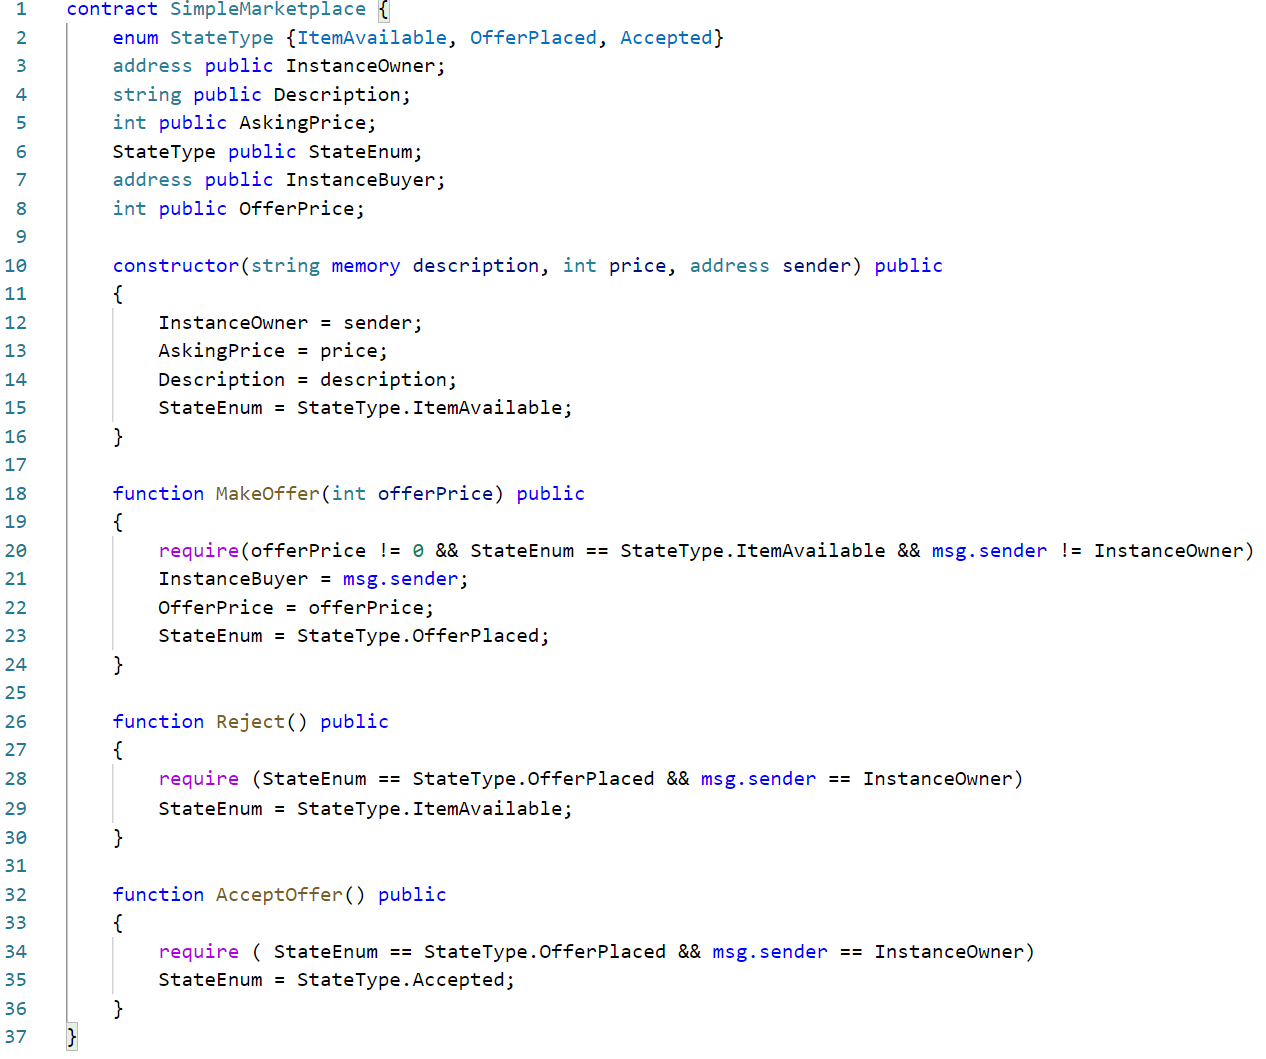
\includegraphics[width=\textwidth]{figs/simple-marketplace.png}}  
    \caption{Contrato Inteligente \texttt{SimpleMarketplace} en Solidity}
    \label{fig:solidity-example}
\end{figure}

\section{Enabledness-Preserving Abstractions}


Una EPA es un Labeled Transition System (LTS) finito que busca abstraer el comportamiento de un contrato inteligente agrupando los estados del contrato en base a cuáles de sus metodos están habilitados \cite{de-caso-epa}.
Las transisiones en estos LTS representan el llamado a una función del contrato, indicando cómo un llamado a una función puede transformar el contrato de un estado abstracto a otro.

Comenzando por un ejemplo, en la figura \ref{fig:epa-example} presentamos la EPA del contrato \texttt{Simple\-Marketplace}.
El estado incial, denominado \textbf{A}, está etiquetado \texttt{init} e indica el estado ``vacío'' previo al llamado al constructor del contrato.
Lo que podemos ver es que luego de ejecutar el método constructor se transiciona en la EPA a un único otro estado, al que llamamos \textbf{B}.
Allí, la etiqueta \texttt{\_MakeOffer} indica que \textcolor{orange}{\texttt{MakeOffer}} es el único método que se encuentra habilitado en \textbf{B}.
La única transición desde \textbf{B}, etiquetada \textcolor{orange}{\texttt{MakeOffer}}, indica lo que ocurre cuando se ejecuta ese método desde ese estado. Como vemos, seguir esa transición nos traslada  al estado \textbf{C}, que es un estado del contrato en el que solamente \textcolor{orange}{\texttt{AcceptOffer}} y \textcolor{orange}{\texttt{Reject}} se encuentran habilitados.
Luego, desde el estado \textbf{C} podemos ejecutar cualquiera de los dos métodos; la transición por \textcolor{orange}{\texttt{Reject}} nos llevará de vuelta al estado \textbf{B} y la transición por \textcolor{orange}{\texttt{AcceptOffer}} nos llevará al estado final \textbf{D}.
Este último, etiquetado ``\texttt{vacio}'' indica que ningún método se encuentra habilitado, por lo que representa el fin forzoso de la ejecución. 



\begin{figure}
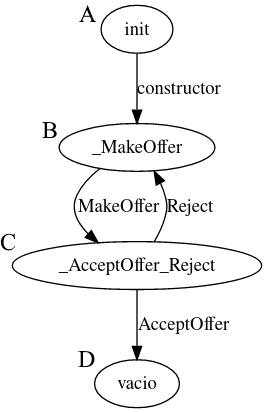
\includegraphics[width=0.3\textwidth]{figs/simple-merketplace-epa.png}  
\caption{EPA de \texttt{SimpleMarketplace}. Las etiquetas en los estados indican los métodos que se encuentran habilitados. Las etiquetas en las transiciones indican el método por el que ocurre la transición.}
\label{fig:epa-example}
\end{figure}

\section{Modelo Formal}
Dado que trabajaremos sobre el código fuente de un contrato escrito en Solidity, nos interesa formalizar qué aspectos del contrato consideraremos relevantes.
Para obtener una discusión más detallada de estas formalizaciones de los artefactos de código, referirse a De Caso et. al.  \cite{de-caso-epa}.
Asimismo, la abstracción presentada del comportamiento de los contratos inteligentes origina en Godoy et. al. \cite{predicate-abstraction-for-smart-contract-validation}.
En esta sección solamente presentamos una compatibilización de los formalismos para facilitar la discusión de las EPAs más adelante.

Dicho eso, llamaremos \textit{configuraciones} a las posibles combinaciones de las variables de estado del contrato y de la blockchain, y notaremos $C$ al conjunto de todas las posibles configuraciones.

\begin{definition}(Formalización de un contrato inteligente)
\label{definicion-smart-contract}
    Definimos a un contrato inteligente como la tupla $SC = \langle M, F, R, inv, init \rangle$ donde:

\begin{itemize}
    \item $M = {m_1, \dots m_n}$ es el conjunto finito de métodos externos definidos en la interfaz del contrato
    \item $F$ es un conjunto de funciones indexadas por $M$. \\
    Para cada $m \in M$, $F_m : C \times \mathds{Z} \rightarrow (C \cup \bot)$ es la implementación del método $m$.
    \item $R$ es un conjunto de precondiciones indexado por $M$.\\
    Para cada $m \in M$, $R_m : C \times \mathds{Z} \rightarrow \{$\textbf{true}, \textbf{false}$\}$ indica si el método $m$ está habilitado para la configuración y parámetros indicados
    \item $inv : C \rightarrow \{$\textbf{true}, \textbf{false}$\}$ indica si una configuración cumple el invariante del contrato
    \item $init : C \rightarrow \{$\textbf{true}, \textbf{false}$\}$ indica si una configuración puede ser resultante de ejecutar el constructor del contrato
\end{itemize}
\end{definition}

Una particularidad presente en los métodos de los contratos inteligentes es que algunas instrucciones como \textcolor{blue}{\texttt{msg.sender}}, \textcolor{blue}{\texttt{msg.value}}, \textcolor{blue}{\texttt{tx.gasprice}} o \textcolor{blue}{\texttt{tx.origin}}
\footnote{\textcolor{blue}{\texttt{msg.value}} indica cuánto Ether está recibiendo el contrato. \textcolor{blue}{\texttt{tx.gasprice}} indica cuánto Ether se le cobra al remitente por cada unidad de gas (cómputo) utilizada y \textcolor{blue}{\texttt{tx.origin}} se refiere a el usuario humano que haya enviado el mensaje que disparó la ejecución actual.} hacen referencia a variables de la blockchain.
Sin embargo podemos modelar estas variables, junto con los parámetros explícitos como input codificable en $\mathds{Z}$ (los números enteros) sin pérdida de generalidad \cite{de-caso-epa}.
La semántica de un contrato la definimos como el siguiente Labeled Transition System:

\begin{definition}\label{definicion-lts}(Semántica de un contrato inteligente)
Dado $SC = \langle M, F, R, inv, init \rangle$ un contrato inteligente, su semántica está provista por el LTS concreto $L_c = \langle \sigma , S_c, S_{0c}, \Delta _c \rangle$ que satisfaga:
\begin{itemize}
    \item $S_c = \{conf | conf \in C \land inv(conf) = \textbf{true}\}$
    \item $S_{0c} = \{conf | conf \in S_c \land init(conf) = \textbf{true}\}$
    \item $\sigma = (F \times \mathds{Z}) \cup \tau$ es el conjunto de todos los posibles llamados a funciones, junto con un elemento $\tau$ que representa un cambio en la blockchain que ocurra de manera independiente al contrato 
    \item $\Delta _c \subseteq S_c \times \sigma \times S_c$ 
    \item $\forall s_1,s_2 \in S_c, m \in M, z \in \mathds{Z} . \\ (s_1,(F_m,z),s_2) \in \Delta _c \iff \bigg( R_m(s_1,z) = \textbf{true} \land   F_m(s_1,z) = s_2 \bigg)$ \\
    $(s_1,\tau,s_2) \in \Delta _c \iff$ un cambio independiente en la blockchain puede llevarnos del estado $s_1$ al estado $s_2$
\end{itemize}
\end{definition}
Notar que para cualquier contrato, el conjunto $S_c$ de estados de su LTS concreto es infinito.
Esto es porque las configuraciones tienen en cuenta variables de la blockchain externas al contrato.
Incluso para contratos donde las configuraciones de las variables internas es finita, siempre habrá infinitas configuraciones de las variables externas.
\\

A la EPA (es decir, el LTS abstracto) la definimos entonces de la siguiente manera:

\begin{definition}\label{definicion-epa}(Enabledness-Preserving-Abstraction) Dado $SC = \langle M, F, R, inv, init \rangle$ un contrato inteligente y $L_c = \langle \sigma , S_c, S_{0c}, \Delta _c \rangle$ su LTS concreto, entonces el LTS asbtracto $L_A = \langle M \cup \hat{\tau} , 2^M, P_0, \Delta _A \rangle$ es una EPA del contrato y $\alpha : S_c \rightarrow 2^M$ es la función de abstracción, donde se cumple que:
\begin{itemize}
    \item $2^M$ es el conjunto de partes de $M$
    \item $\forall s \in S_c \: . \:
    \alpha(s) = \{m | m \in M \land \exists z \in \mathds{Z} . R_m(s,z) = \textbf{true}\}$
    \item $P_0 = \{\alpha(s_0) | s_0 \in S_{0c} \}$
    \item $\forall s_1,s_2 \in S_c, m \in M, z \in \mathds{Z} . \\ (s_1,(F_m,z),s_2) \in \Delta _c \Rightarrow (\alpha(s_1),R_m,\alpha(s_2)) \in \Delta _A$ \\ 
    $(s_1,\tau,s_2) \in \Delta _c \Rightarrow (\alpha(s_1),\hat{\tau},\alpha(s_2)) \in \Delta _A$
\end{itemize}
\end{definition}

El conjunto de estados de la \textit{EPA} es $2^M$ (el conjunto de partes de las precondiciones). 
La \textit{función de abstracción} de los estados $s_c$ del LTS concreto a los estados abstractos es $\alpha (s_c) = $ ``el conjunto de métodos cuyas precondiciones son satisfechas por $s_c$''.
Una transición en la EPA entre los estados $s$ y $s'$ etiquetada con el método $m$ significa que existen algún estado concreto $s_c$ y un valor de entrada $z$ para los que $\alpha(s_c) = s$ y  $F_m(s,z)=s_c'$ con $\alpha(s_c') = s'$.
Es decir que algún llamado de $m$ a un estado que se abstrae a $s$ nos da de resultado otro estado que se abstrae a $s'$.
Una transición de $s$ a $s'$ etiquetada  con $\hat{\tau}$, la versión abstracta de $\tau$, indica que existe un estado concreto $s_c$ con $\alpha(s_c) = s$ y que puede ocurrir $\alpha (\tau (s_c)) = s'$.


\chapter{Manticore}
En esta sección haremos un breve repaso de las funcionalidades provistas por \texttt{Manticore}.
Luego podremos discernir dadas estas funcionalidades la mejor estrategia para utilizar \texttt{Manticore} como el back end de la construcción de EPAs.
Toda esta sección se refiere a la versión de \texttt{Manticore 0.3.7}.

\texttt{Manticore} es un proyecto desarrollado por \texttt{TrailOfBits} lanzado en 2017.
Es una herramienta de ejecución simbólica, implementada en Python, que soporta análisis para diversas plataformas: EVM, bytecode nativo (arquitecturas \texttt{x86}, \texttt{x86\_64}, \texttt{aarch64} y \texttt{ARMv7}) y WASM.
Principalmente funciona como un motor de ejecución simbólica programable (mediante APIs en Python), aunque también incluye una herramienta plug-and-play por línea de comandos, y existe un proyecto que intenta integrar la herramienta con una interfaz gráfica, \texttt{ManticoreUI} \cite{manticoreUI} que nunca se lanzó.

\section{Herramienta por Línea de Comandos}

El comportamiento por defecto de la herramienta de línea de comandos varía mucho dependiendo de la plataforma a la que es aplicada, pero en general busca explorar todos los caminos de ejecución factibles en el código fuente provisto, utilizando valores simbólicos para cada valor generalmente introducido por usuarios.
Luego, por cada camino explorado, genera un caso de test (es decir, genera un valor concreto que fuerze el camino para cada valor ``input'' simbólico).
Además, la exploración de los caminos incluye el seguimiento de algunas propiedades interesantes por defecto, dependientes de la plataforma.
Para los binarios nativos, por ejemplo, registra el conjunto (total) de instrucciones visitadas, y registra para cada caso de test el número y la traza exacta de instrucciones ejecutadas.

En el caso de programas de la EVM, la herramienta por consola funciona con código fuente Solidity (no acepta precompilados).
Para explorar caminos de ejecución la herramienta toma los métodos externos del contrato y los ejecuta (en cualquier orden) hasta alcanzar 100\% de line coverage o, dentro de un límite si es que se introdujo uno, hasta cubrir todo el espacio de secuencias de llamados a métodos externos.
De no alcanzar ninguno de estos dos criterios, termina el análisis por time out.
La herramienta cuenta con una batería de \texttt{detectors} que registran eventos de  interés específico a Ethereum, como la presencia de integer overflows, la ejecución de opcodes inválidos, la lectura de memoria o storage no inicializado, bugs de reentrancy o la ejecución de ciertas instrucciones específicas con parámetros controlados por el usuario.
Estos \texttt{detectors} se encuentran apagados por defecto, al igual que por defecto se descartan caminos que incluyan el rollback de una transacción.
Esto significa que, por ejemplo, para realizar una simple búsqueda de incumplimiento de una aserción (la instrucción \textcolor{blue}{\texttt{assert}} en Solidity), es preciso activar el modo detallado (\texttt{--thorough-mode}) de la herramienta.

\section{Manticore-Verifier}
Manticore cuenta con otra herramienta por consola de comandos de análisis de smart contracts denominada \texttt{manticore-verifier}.
Permite marcar ciertos métodos externos como ``invariantes'' que la herramienta luego busca falsificar.
Una fortaleza de esta herramienta es que la sintaxis para marcar los invariantes es la misma que la utilizada por \texttt{Echidna}, un fuzzer desarollado también por \texttt{TrailOfBits} \cite{echidna}, permitiendo el análisis por ambas herramientas con una única intervención manual.

\section{Arquitectura}
La arquitectura de Manticore se organiza en tres partes:
\begin{itemize}
    \item El mecanismo central de ejecución simbólica
    \item Los módulos que implementan la simulación de cada una de las plataformas soportadas (Ethereum, \texttt{x86}, etc)
    \item SMT solvers externos
\end{itemize}

Por defecto, la instalación de Manticore incluye una instalación del \texttt{Z3 Theorem Prover}, un SMT solver desarrollado por Microsoft Research desde 2012 \cite{z3TheoremProver}.
Sin embargo, Manticore puede integrarse con cualquier SMT solver que se conforme a la interfaz definida por \texttt{SMTLIB2} \cite{smtlib2}, como lo es por ejemplo también \texttt{Yices} \cite{yices}, otro SMT solver open source.

El mecanismo central de ejecución simbólica de Manticore está compuesto por varios módulos de Python: \texttt{\textbf{smtlib}}, \texttt{\textbf{manticorebase}}, \texttt{\textbf{plugin}}, \texttt{\textbf{state}}, \texttt{\textbf{worker}} y \texttt{\textbf{workspace}}, representados en la figura \ref{fig:core-modules}.

\begin{figure}
    \centering
    {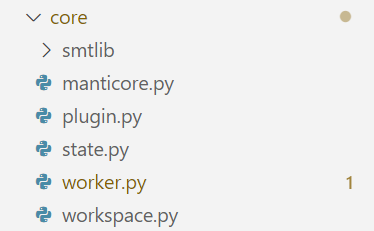
\includegraphics {figs/core-architecture-manticore.png}}
    \caption{Módulos que componen el mecanismo central de ejecución simbólica de Manticore}
    \label{fig:core-modules}
\end{figure}

\texttt{\textbf{smtlib}} provee a los demás módulos de la aplicación APIs para generar y manipular variables, expresiones y constraints simbólicas, y para realizar consultas de (in)satisfacibilidad sobre las expresiones simbólicas generadas, delegando estas consultas en última instancia al SMT solver externo.
Los módulos \texttt{\textbf{manticorebase}} y \texttt{\textbf{state}} implementan en conjunto el mecanismo central de ejecución simbólica de Manticore asumiendo lo mínimo posible sobre las instrucciones emuladas \footnote{Es decir, sobre la plataforma que use el programa que se está analizando}.
Por último, \texttt{\textbf{worker}} y \texttt{\textbf{workspace}} sirven de auxiliares que soportan los aspectos de perstistencia, entrada/salida y multithreading, entre otros, de la aplicación.
El módulo \texttt{\textbf{plugin}} provee una API de \textit{callbacks} que otorgan acceso al estado interno emulado en distintos momentos de la ejecución.
Este módulo es una parte central de la API programable accesible al usuario de Manticore, pero también es la manera en la que la aplicación base puede realizar sus análisis de coverage, etc.

La abstracción principal para la ejecución simbólica utilizada por Manticore es la del objeto \textcolor{cyan}{\texttt{state}}.
Un \textcolor{cyan}{\texttt{state}} representa, habiendo realizado un camino de ejecución particular, el estado del programa emulado hasta cierto punto.
Los \textcolor{cyan}{\texttt{state}} son responsables de conocer cuáles son los próximos pasos en su ejecución, cuál es el conjunto de variables simbólicas que existieron en su ejecución, y qué conjunto de fórmulas deben satisfacerse.
Asimismo, cada \textcolor{cyan}{\texttt{state}} individual cuenta con una instancia entera emulada del estado del programa (en el caso de Ethereum, esto es simulaciones enteras de blockchains).
Por otro lado, el estado global de la aplicación (mantenido por el módulo \texttt{\textbf{manticorebase}}) consiste simplemente en una colección de \textcolor{cyan}{\texttt{state}}.

\section{API programable}
\label{sec:api-manticore}
La principal API presentada al usuario permite manejar el conjunto global de \textcolor{cyan}{\texttt{state}}, siempre ``entre medio'' de la ejecución de métodos del contrato (es decir, antes de comenzar a ejecutarlos o después de que terminen, pero no durante).
Los principales métodos de la API permiten realizar acciones globales como introducir nuevas constraints, ejecutar métodos de un smart contract, deployear un contrato nuevo, o iniciar la generación de casos de test a partir de los \textcolor{cyan}{\texttt{state}}.
Además, permiten acceder a \textcolor{cyan}{\texttt{state}} individuales (siempre y cuando no estén corriendo) y leer y/o modificar los elementos simbólicos de su estado.
Sin embargo, al menos mediante la API expuesta, no es posible expandir el camino de ejecución de sólo algunos \textcolor{cyan}{\texttt{state}}.
Esto siempre debe hacerse mediante la ejecución de métodos externos al nivel más alto, afectando a todos los \textcolor{cyan}{\texttt{state}} \footnote{Veremos que esta limitación guió el diseño del algoritmo presentado en la sección \ref{sec:algoritmo-aternativo}}.

Por otro lado los callbacks como los del módulo
\texttt{\textbf{plugin}} permiten interactuar con los \textcolor{cyan}{\texttt{state}} mientras estos se ejecutan.
Los callbacks pueden suscribirse a cualquiera de los eventos publicados nativamente por la aplicación, que son de naturaleza muy amplia y granularidad diversa, y no simplemente eventos que modifiquen el estado de los \textcolor{cyan}{\texttt{state}}.
Algunos de los eventos pueden categorizarse en:
\begin{itemize}
    \item eventos de \textcolor{cyan}{\texttt{state}} (\texttt{will\textbackslash did\_fork\_state, will\textbackslash did\_terminate\_state})
    \item eventos de smt (\texttt{will\textbackslash did\_solve})
    \item eventos de plataforma (\texttt{will\textbackslash did\_open\_transaction},\\ \texttt{will\textbackslash did\_evm\_read\_storage})
\end{itemize}
Los callbacks pueden resultar útiles para debugear o mantener el registro de propiedades, pero también es posible utilizarlos para modificar el estado de la ejecución en vivo.




\chapter{Construcción de EPAs mediante ejecución simbólica}
En las últimas dos secciones vimos las formalizaciones relacionadas con las EPAs y las capacidades de Manticore.
A continuación, presentaremos dos algoritmos para la construcción de EPAs.
El algoritmo clásico es presentado, con algunas diferencias de notación, como fue presentado por De Caso et. al en 2013 \cite{de-caso-epa}.
El algoritmo novedoso hace uso específicamente de ejecución simbólica y, al haber sido diseñado para Manticore, se adapta a las peculiaridades mencionadas en la sección anterior.

\section{Construcción clásica de EPAs}
\label{sec:algoritmo-clasico}
Tradicionalmente, existe un algoritmo genérico para la construcción de \textit{EPAs} de artefactos de código.
Por cuestiones de notación, para ver el algoritmo de generación de EPAs es conveniente definir el siguiente predicado presentado por De Caso et. al \cite{de-caso-epa} sobre las configuraciones dado un conjunto de precondiciones de un contrato:

\begin{definition}[Predicado de un conjunto de métodos]
    Dados un contrato $SC = \langle M, F, R, inv, init \rangle$ y un conjunto de metodos, $\mathcal{M} \subseteq M$, definimos $pred_\mathcal{M} : \mathcal{C} \rightarrow \{\textbf{true}, \textbf{false}\}$ como
    \[pred_\mathcal{M}(c) \iff inv(c) \land \bigwedge\limits_{m \in \mathcal{M}} \exists p \in \mathds{Z} . R_m(c,p) \land \bigwedge\limits_{   m \notin \mathcal{M}} \nexists p \in \mathds{Z} . R_m(c,p)\]
\end{definition}
El algoritmo, que presentamos a continuación, genera la porción de la EPA que es alcanzable desde $P_0$ (los estados iniciales), realizando \textit{Breadth-First-Search} en el grafo de las transiciones \cite{de-caso-epa}.

\begin{algorithm}[H]
    \caption{Construcción de EPAs}
    \hspace*{\algorithmicindent} \textbf{Input} $SC = \langle M, F, R, inv, init \rangle$ contrato \\
    \hspace*{\algorithmicindent} \textbf{Output} La \textit{EPA} $L_A =\langle \Sigma, S, P_0, \Delta \rangle$
    \begin{algorithmic}[1]
        \State $\Sigma = M$; $S = \emptyset$
        \State $\Delta(s,m) = \emptyset \quad \forall s \in 2^R, m \in M$
        \State $\mathcal{M}^- = \{m \in M | \forall c \: . \: init(c) \Rightarrow \nexists p \in \mathds{Z} \: . \: R_m(c,p)\}$
        \State $\mathcal{M}^+ = \{m \in M | \forall c \: . \: init(c) \Rightarrow \exists p \in \mathds{Z} \: . \: R_m(c,p)\}$
        \State $P_0^c = \{\mathcal{M} \in \#M | \mathcal{M}^+ \subseteq \mathcal{M} \land \mathcal{M}^- \cap \mathcal{M} = \emptyset \}$
        \State $P_0 = \{\mathcal{M} \in P_0^c | \exists c . init(c) \land pred_\mathcal{M}(c) \}$
        \State $W =$ Cola con los elementos de $P_0$
        \While{hay un conjunto $\mathcal{M}$ en la cabeza de $W$}
        \State $S = S \cup \{\mathcal{M}\}$
        \For{$m \in \mathcal{M}$}
        \State $\mathcal{N}^- = \{n \in M | \forall c \in \mathcal{C}, p \in \mathds{Z} \: . \: pred_\mathcal{M}(c) \land R_m(c,p) \Rightarrow \nexists p^\prime \in \mathds{Z} \: . \: R_n(F_m(c,p),p^\prime)\}$
        \State $\mathcal{N}^+ = \{n \in M | \forall c \in \mathcal{C}, p \in \mathds{Z} \: . \: pred_\mathcal{M}(c) \land R_m(c,p) \Rightarrow \exists p^\prime \in \mathds{Z} \: . \: R_n(F_m(c,p),p^\prime)\}$
        \State $S^C = \{\mathcal{N} \in \#M | \mathcal{N}^+ \subseteq \mathcal{N} \land \mathcal{N}^- \cap \mathcal{N} = \emptyset\}$
        \For{$\mathcal{N} \in S^C$}
        \If{$ \exists c \in \mathcal{C} \: . \: pred_\mathcal{M} (c) \land \exists p \in \mathds{Z} \: . \: R_m(c,p) \land pred_\mathcal{N}(F_m(c,p)) $}
            \State $\Delta (\mathcal{M},m) = \Delta (\mathcal{M},m) \cup \mathcal{N}$
            \If{$\mathcal{N} \notin S \land \mathcal{N} \notin W$}
            \State $W.push(\mathcal{N})$
            \EndIf
            \EndIf
            \EndFor
            \EndFor
            \EndWhile
            \State \Return $\langle \Sigma, S, P_0, \Delta \rangle$
    \end{algorithmic}
\end{algorithm}

Aquí, calcular los conjuntos $\mathcal{M}^-$, $\mathcal{M}^+$, $\mathcal{N}^-$ y $\mathcal{N}^+$ es una optimización que permite reducir la cantidad de transiciones candidatas de la EPA \cite{de-caso-epa}.

Decidir si una transición pertenece o no la EPA, como está planteado en el algoritmo, es resolver problemas de validez de fórmulas de primer orden.
Esto en general es indecidible, sin embargo la sugerencia principal consiste en transformar estas preguntas de validez de fórmulas de primer orden en problemas de alcanzabilidad de código, dado que se espera que las precondiciones y los invariantes definidos en la formalización~\ref{definicion-smart-contract} estén debidamente implementados en el contrato.

En general, por optimizaciones de gas, es común que en los métodos externos los contratos definan las precondiciones explícitamente mediante instrucciones \textcolor{magenta}{\texttt{require}}, como en el contrato ejemplo \ref{fig:solidity-example} \texttt{SimpleMarketplace}.
Dado que los inputs externos nunca garantizan estar bien formados, resulta menos costoso para el contrato abortar estas ejecuciones lo antes posible en lugar de hacerlas avanzar hasta llegar a un estado de error.
Sin embargo, debido a que no se espera que sea posible generar instancias que no satisfagan el invariante, por el mismo motivo de ahorro de gas, no es usual contar con una implementación explícita del invariante en el código fuente del contrato.
Tenerlo implicaría ejecutar código que se espera que dé siempre el mismo resultado, por lo que resulta más eficiente no hacerlo.

\section{Algoritmo alternativo}
\label{sec:algoritmo-aternativo}
Implementar el invariante del contrato, además de no ser una práctica estándar, es a menudo exigente para el programador, y es también una actividad propensa a errores.
Sin embargo, es importante en la definición~\ref{definicion-lts} de la semántica de un contrato inteligente la  presencia del invariante.
Intentar construir EPAs incluyendo estados que no satisfagan el invariante suele producir abstracciones demasiado sobreaproximadas \cite{de-caso-epa}.
Por eso, en continuación del trabajo presentado por Godoy et al. \cite{predicate-abstraction-for-smart-contract-validation}, trabajaremos construyendo las EPAs a partir de las precondiciones explícitas dadas por las declaraciones \textcolor{magenta}{\texttt{require}} al comienzo de los métodos, y haciendo uso  del invariante implícito dado por los métodos mismos del contrato.

Trabajemos con la acepción de que un contrato es correcto si la ejecución de todos sus métodos preservan el invariante si se satisfacen las precondiciones del método.
La idea es que bajo la asunción de que un contrato es correcto, ejecutar cualquier sucesión de métodos del contrato con parámetros válidos (es decir, que satisfagan las precondiciones) genera instancias que satisfacen el invariante.
Esto significa que explorar cadenas de transacciones que comienzen por el constructor siempre considera estados que satisfacen el invariante, siempre y cuando cada llamado individual a métodos cumpla las precondiciones correspondientes.
Entonces, es posible asumir que se satisface el invariante si se presenta una traza de llamados válidos a métodos que comienza por el constructor.

Por otro lado, si todos los métodos de un contrato implementan explícitamente sus precondiciones, podemos decir aún mas.
Si este es el caso entonces es imposible que ningún llamado a un método genere un estado inválido.
En su lugar, un llamado que no satisfaga las precondiciones del método será revertido.
De esta manera, \textit{cualquier} traza de métodos que comienze por el constructor genera una instancia del contrato que satisface el invariante, si los métodos implementan explícitamente sus precondiciones.

En esta sección presentamos el algoritmo que construye EPAs haciendo uso de una herramienta de ejecución simbólica, siguiendo la idea esbozada anteriormente para mantener el análisis en estados que satisfagan el invariante.
Dado que trabajaremos asumiendo que no hay acceso explícito al invariante, la nueva formalización que utilizaremos para los contratos inteligentes es la siguiente:

\begin{definition}(Formalización laxa de un contrato inteligente)
    \label{definicion-laxa-smart-contract}
    Definimos a la versión laxa de un contrato inteligente como la tupla $SC = \langle M, F, R, Constructor \rangle$ donde:
    \begin{itemize}
        \item $M, F$ y $R$ son iguales a la definición original
        \item $inv$ no forma parte de $SC$ porque asumimos que se preserva luego de cada llamado a $F_m(c,p)$ independientemente de si $R_m(c,p) = \textbf{true}$
        \item $Constructor \in M$ reemplaza el predicado $init$ y representa un método del contrato que genera las instancias iniciales.
    \end{itemize}
\end{definition}
El LTS concreto (la semántica) y el LTS abstracto (la EPA) de smart contracts que usan esta definición pueden formalizarse de manera análoga a las secciones anteriores.
Por cuestiones de notación, introduciremos algunas funciones sobre los caminos posibles en los métodos de un contrato:
\begin{definition}[Conjunto de posibles caminos de ejecución de una secuencia de funciones]
    Dados un contrato $SC = \langle M, F, R, Constructor \rangle$ definimos la función \texttt{paths\_of} que opera en el dominio de las secuencias de funciones $f_1, f_2, \cdots f_k$ tales que $\forall i, f_i \in F \cup R$:
    \begin{multline}
        \texttt{paths\_of}(f_1, f_2, \cdots f_k) = \{p \: | \: p \text{ es una secuencia de instrucciones del código fuente de SC} \\
        \text{que podría ser un camino que toma la ejecución de } f_1, f_2, \cdots f_k \}
    \end{multline}
\end{definition}
En particular, \texttt{paths\_of} se refiere al conjunto de caminos que son efectivamente factibles.
Es decir, no se consideran caminos de ejecución para los que no exista una serie de inputs que obligan a recorrerlos.
\begin{definition}[Resultado simbólico del camino de ejecución en una secuencia de funciones]
    Dados un contrato $SC = \langle M, F, R, Constructor \rangle$ definimos la función \texttt{sym\_res\_of} que opera en el dominio de los caminos de secuencias de funciones:
    \begin{multline}
        \texttt{sym\_res\_of}(p) = \text{le asocia un valor simbólico a cada función que fue llamada en }p
    \end{multline}
\end{definition}

A continuación usaremos la notación ``$\mathcal{M}=sy$'' donde $\mathcal{M}$ es un estado abstracto de la EPA y $sy$ uno de los estados simbólicos mencionados anteriormente.
Esta notación la usaremos para referirnos a la ``fórmula de compatibilidad'' entre estos dos.
Brevemente, recordemos que un estado de la EPA $\mathcal{M}$ es un subconjunto de los métodos del contrato, y representa los estados concretos en los que los métodos contenidos en el subconjunto se encuentran habilitados, y los demás se encuentran deshabilitados.
Podremos decir que para un camino de ejecución $p$ de las funciones $R_{m\_1},R_{m\_2} \cdots R_{m\_n}$ el resultado simbólico de $p$, $sy = \texttt{symb\_res\_of}(p)$ es compatible con $\mathcal{M}$ sí y sólo sí para cada $R_m$, el resultado de $R_{m\_i}$ en $sy$ es \textbf{true} $\iff m\_i \in \mathcal{M}$.

Consideremos el siguiente ejemplo para el contrato \texttt{Simple\allowbreak Marketplace}:
Sean $\mathcal{M} = \{MakeOffer, Reject\}$ y $p_1$ que representa un camino hasta cierto punto de \texttt{SimpleMarketplace}.
Sea $p_2 \in \texttt{paths\_of}(R_{MakeOffer}; R_{AcceptOffer}; R_{Reject})$ que representa un camino posible de ejecutar las precondiciones del contrato.
Además, sea $sy = \texttt{symb\_res\_of}(p_1;p_2)$, donde con ``$;$'' notamos la concatenación de caminos, tal que los resultados de las precondiciones en $sy$ son $\{R_{MakeOffer} = r_1$, $R_{AcceptOffer} = r_2$, $R_{Reject} = r_3\}$.
La fórmula de compatibilidad entre $\mathcal{M}$ y $sy$ será $\Phi = (r_1 = \textbf{true} \land r_2 = \textbf{false} \land r_3 = \textbf{true} \land sy)$ y significa que en la ejecución de $(R_{MakeOffer}; R_{AcceptOffer}; R_{Reject})$ existen valores de entrada que recorren $p_1;p_2$ y que los resultados dan \textbf{true} para \textcolor{orange}{\texttt{MakeOffer}} y \textcolor{orange}{\texttt{Reject}} y false para \textcolor{orange}{\texttt{AcceptOffer}}.
Dicho de otra manera, esto es que existen parámetros de entrada que generan un estado que se abstrae a $\mathcal{M}$ luego de la ejecución de $p_1$.
Luego, esto quiere decir que si la fórmula $\Phi$ es satisfacible, entonces tenemos garantía de que luego de ejecutar $p_1$ el contrato \textit{puede} encontrarse en un estado que se abstrae a $\mathcal{M}$.
Por otro lado la no satisfacibildad de $\Phi$ indicaría que es imposible llegar al estado de la epa $\mathcal{M}$ luego de ejecutar $p1$.
El algoritmo para expresar la fórmula de compatibilidad entre $p_1$ y $sy$ es el siguiente:

\begin{algorithm}[H]
    \captionsetup{belowskip=0pt}
    \caption{Operador ``$=$'' entre estados de una EPA y resultados simbólicos (ecuación de compatibilidad)}
    \hspace*{\algorithmicindent} \textbf{Input} $SC = \langle M, F, R, Constructor \rangle$ contrato \\
    \hspace*{\algorithmicindent} \textbf{Input} $\mathcal{M}$ un estado de la EPA de $SC$ \\
    \hspace*{\algorithmicindent} \textbf{Input} $sy$ resultado simbolico de una ejecución de $SC$ \\
    \hspace*{\algorithmicindent} \textbf{Output} La fórmula de compatibilidad $\Phi$
    \begin{algorithmic}[1]
        \State $\Phi = sy$
        \For{$m \in M$}
        \State $res_m =$ valor de retorno de la última aparición de $R_m$ en $sy$
        \If{$m \in \mathcal{M}$}
        \State $\Phi = \Phi \land (res_m == \textbf{true})$
        \Else
        \State $\Phi = \Phi \land (res_m == \textbf{false})$
        \EndIf
        \EndFor
        \State \Return $\Phi$
    \end{algorithmic}
\end{algorithm}

Utilizando estas notaciones, podemos presentar el algoritmo\ref{alg:alternativo} que explora la porción de la EPA que es alcanzable desde $P_0$, sin acceso al invariante y haciendo uso de ejecución simbólica.
Este algoritmo realiza una versión	modificada de \textit{Depth-First-Search} en el grafo de las transiciones, explorando varias aristas del grafo a la vez.
En particular, en cada iteración del ciclo principal este algoritmo agrega múltiples transiciones a la EPA etiquetadas por un mismo método.
La exploración siempre se realiza a partir del conjunto de estados de la EPA ``$S_{current}$'' que en cada iteración se actualiza con el conjunto de estados en los que puede resultar la ejecución del último método.
Cuando esta exploración llega a un punto muerto, se retrocede usando la pila del \textit{DFS} hasta otro punto en el que queden llamados de métodos sin explorar.
\begin{algorithm}[H]
\captionsetup{belowskip=0pt}
\caption{Construcción de EPAs mediante ejecución simbólica}
 \hspace*{\algorithmicindent} \textbf{Input} $C = \langle M, F, R \rangle$ contrato \\
 \hspace*{\algorithmicindent} \textbf{Output} La \textit{EPA} $L_A =\langle \Sigma, S, P_0, \Delta \rangle$
 \begin{algorithmic}[1]
\State $\Sigma = M$
\State $S = \emptyset$ $;P_0 = \emptyset$
\State $\Delta(s,m) = \emptyset \quad \forall s \in 2^R, m \in M$
\State $Paths_{pre} = \{p | p$ es un posible camino de ejecución de $F_{Constructor};R\_1;R\_2; \dots R\_n\}$
\State $Symb_{pre} = \{$resultado simbólico luego de ejecutar $p | p \in Paths_{pre} \}$ 
\State $P_0 = \{s \in 2^R | \exists sy \in Symb_{pre} \: . \: SAT(sy= s)\}$
\State $S_{current } = P_0$
\State $marcados = \emptyset$
\State $W =$ Pila vacía ;$W.$Push$((S_{current},Symb_{pre}))$
\While{$W . $NotEmpty$()$}
    \State $S =$ Update con $S_{current }$
    \If{$\exists m \in M\: . \: \{s \in S_{current } | m \in s \land (s,m) \notin marcados\} \neq \emptyset$} 
        \State Elegir tal $m$
        \State $Paths_{post\_m} = \{p | p$ es un posible camino de ejecución de $F_m;R\_1;R\_2; \dots R\_n\}$
        \State $Symb_{post} = \{$resultado simbólico luego de ejecutar $p1;p2 \:|\: p1 \in Paths_{pre} \land p2 \in Paths_{post\_m} \} $
        \State $S_{next} = \emptyset$
        \For{$\{s_1 \in S_{current } | m \in s_1 \land (s_1,m) \notin marcados\}$}
            \State $marcados \pluseq \{(s_1,m)\}$
            \State  $\Delta(s_1,m) = \{s_2 \in 2^R | \exists sy_1 \in Symb_{pre}, sy_2 \in Symb_{post\_m} \: . \: SAT(sy_1= s_1 \land sy_2 = s_2)\}$ 
            \State $S_{next} = \Delta(s_1,m)$
        \EndFor
        \State $S_{current } = S_{next}$
        \State $Symb_{pre} = Symb_{post}$
        \State $Paths_{pre} = (Paths_{Pre};$ $Paths_{Post})$ 
        \State $W.$Push$((S_{current },Symb_{pre}))$
    \Else
        \State $(S_{current },Symb_{pre}) = W.$Pop$()$
    \EndIf
\EndWhile
\State \Return $\langle \Sigma, S, P_0, \Delta \rangle$
\end{algorithmic}
\end{algorithm}
%\begin{tcolorbox}[blanker,
%        float=htb!,
%        grow to left by=1.5cm,
%        grow to right by=1.2cm,
%        top=-1.2cm,
%        bottom=-0.8cm]
%    \begin{algorithm}[H]
\captionsetup{belowskip=0pt}
\caption{Construcción de EPAs mediante ejecución simbólica}
 \hspace*{\algorithmicindent} \textbf{Input} $C = \langle M, F, R \rangle$ contrato \\
 \hspace*{\algorithmicindent} \textbf{Output} La \textit{EPA} $L_A =\langle \Sigma, S, P_0, \Delta \rangle$
 \begin{algorithmic}[1]
\State $\Sigma = M$
\State $S = \emptyset$ $;P_0 = \emptyset$
\State $\Delta(s,m) = \emptyset \quad \forall s \in 2^R, m \in M$
\State $Paths_{pre} = \{p | p$ es un posible camino de ejecución de $F_{Constructor};R\_1;R\_2; \dots R\_n\}$
\State $Symb_{pre} = \{$resultado simbólico luego de ejecutar $p | p \in Paths_{pre} \}$ 
\State $P_0 = \{s \in 2^R | \exists sy \in Symb_{pre} \: . \: SAT(sy= s)\}$
\State $S_{current } = P_0$
\State $marcados = \emptyset$
\State $W =$ Pila vacía ;$W.$Push$((S_{current},Symb_{pre}))$
\While{$W . $NotEmpty$()$}
    \State $S =$ Update con $S_{current }$
    \If{$\exists m \in M\: . \: \{s \in S_{current } | m \in s \land (s,m) \notin marcados\} \neq \emptyset$} 
        \State Elegir tal $m$
        \State $Paths_{post\_m} = \{p | p$ es un posible camino de ejecución de $F_m;R\_1;R\_2; \dots R\_n\}$
        \State $Symb_{post} = \{$resultado simbólico luego de ejecutar $p1;p2 \:|\: p1 \in Paths_{pre} \land p2 \in Paths_{post\_m} \} $
        \State $S_{next} = \emptyset$
        \For{$\{s_1 \in S_{current } | m \in s_1 \land (s_1,m) \notin marcados\}$}
            \State $marcados \pluseq \{(s_1,m)\}$
            \State  $\Delta(s_1,m) = \{s_2 \in 2^R | \exists sy_1 \in Symb_{pre}, sy_2 \in Symb_{post\_m} \: . \: SAT(sy_1= s_1 \land sy_2 = s_2)\}$ 
            \State $S_{next} = \Delta(s_1,m)$
        \EndFor
        \State $S_{current } = S_{next}$
        \State $Symb_{pre} = Symb_{post}$
        \State $Paths_{pre} = (Paths_{Pre};$ $Paths_{Post})$ 
        \State $W.$Push$((S_{current },Symb_{pre}))$
    \Else
        \State $(S_{current },Symb_{pre}) = W.$Pop$()$
    \EndIf
\EndWhile
\State \Return $\langle \Sigma, S, P_0, \Delta \rangle$
\end{algorithmic}
\end{algorithm}
%\end{tcolorbox}

La decisión de explorar los estados de la EPA de esta manera conjunta se debe a las capacidades de la API programable de Manticore.
Al ejecutar un método, debemos ejecutarlo en todos los caminos hasta el momento.
Por este motivo es que exploramos las transiciones desde todos los estados del conjunto ``$S_{current}$'' cada vez, en lugar de realizar una exploración más tradicional en el grafo de transiciones.

Por último, podemos señalar que para garantizar \textit{soundness} de las EPAs generadas, lo tradicional es consultar por la insatisfacibilidad de que una transición pertenezca a la EPA, e incluirla en el resultado en cualquier caso en el que no se pueda demostrar esto.
Sin embargo, en este caso sólo estamos incluyendo las transiciones para las que tengamos una demostración de su existencia.
Esta decisión, aunque discutible, fue prinicipalmente tomada para aprovechar la funcionalidad de generación de casos de test concretos de Manticore.

%El estado inicial y la función de transición comienzan vacíos.
%El conjunto ${Paths_{pre}}$ contiene todos los caminos posibles que puede tomar la ejecución del constructor seguida por la ejecución de las precondiciones de los métodos.
%Si llamamos $init$ al estado (simbólico) luego de ejecutar $F_{Constructor}$, en $Symb_{pre}$ hay para cada uno de los caminos en $Path_{pre}$ una expresión que representa el resultado de la ejecución realizada. Esa expresión es de la forma $(R_1(init) = r_1 , R_2(init) = r_2 \cdots , R_n(init) = r_n)$ .
%Luego, puede calcularse $P_0$ mediante una sucesión de preguntas de satisfacibilidad de fórmulas.
%En particular, para cada expresión $sy \in Symb_{pre}$, nos interesa saber con qué estado de la EPA es consistente $sy$.

%Habiendo determinado $P_0$, el algoritmo marca $S_{current}$ como el conjunto de estados de la EPA con los que se corresponde $Symb_{pre}$, y agrega ambos a la pila $W$, que representa conjuntos de estados de la EPA por visitar.
%Para continuar la exploración desde $S_{current}$, se elige uno de los métodos que esté habilitado en alguno de los estados de $S_{current}$ y no se haya explorado ya.
%Luego, para cada estado $s \in S_{current}$ que permite la ejecución de $m$, se calculan los nuevos estados a los que se puede llegar ejecutando $m$, de manera similar a la que se calcula $P_0$.

%El conjunto $Symb_{post}$ de la línea 15 representa los resultados de continuar la ejecución donde la había dejado $Symb_{pre}$.
%En la línea 19, donde se calculan las próximas transiciones, es necesario revisar no sólo la satisfacibildad de que el estado simbólico nuevo sea compatible con el estado de la EPA objetivo, sino que es necesario que aún se mantenga la compatibilidad entre el estado simbólico viejo y el estado de la EPA desde el que se está transisionando.
%Esto es porque las expresiones en $Symb_{pre}$ pueden ser compatibles con $s_1$, pero puede ocurrir una contradicción al pedir que $Symb_{post}$ sea compatible con $s_2$ también.
%De no exigir esto, consideraríamos que valores de entrada que permiten alcanzar $s_2$ pero que nunca alcanzaban $s_1$ previamente indican una transición entre $s_1$ y $s_2$.

\section{Limitaciones}
\label{sec:subaproximacion}
La mayor evidente diferencia entre el algoritmo presentado en la seccion \ref{sec:algoritmo-aternativo} y el algoritmo clásico es que en lugar de poder explorar transiciones entre estados completamente abstractos, la manera en la que explora las transiciones de la EPA implica que sólo está considerando ciertos caminos de métodos al evaluar cada transición.
Esto se debe a que en cada paso selecciona un par (método, estado abstracto) que no haya explorado ya, pero la exploración considera todos los estados posibles que puedan abstraerse al estado abstracto.
En cambio, sólo puede considerarse un subconjunto de los estados que la herramienta pudo alcanzar hasta ese momento.

Consideremos el siguiente ejemplo, el contrato \texttt{BoundedStack}, cuyo código podemos ver en el fragmento de código \ref{code:solidity-bounded-stack}.
Este contrato consiste en una simple implementación de una pila como estructura de datos, con la peculiaridad de que la pila cuenta con un tamaño máximo.
El contrato tiene sólo dos métodos externos: \textcolor{orange}{\texttt{push}} y \textcolor{orange}{\texttt{pop}}.
La EPA de este contrato por otro lado también es bastante sencilla, y la podemos ver en la imagen \ref{fig:bounded-stack-epa}.
Por fuera de los estados \textbf{init} y \textbf{vacio}, contamos con solo tres estados alcanzables, que son \textbf{\_push}, \textbf{\_pop} y \textbf{\_push\_pop}.
El estado \textbf{\_push} se corresponde con la pila vacía, y es el que se produce al desplegar el contrato o luego de ejecutar \textcolor{orange}{\texttt{pop}} reiteradas veces.
Cuando la pila tiene elementos pero no está llena se encuentra en el estado \textbf{\_push\_pop}, al que se puede llegar tanto desde sí mismo, como desde \textbf{\_push} y desde \textbf{\_pop}.
Finalmente, el estado \textbf{\_pop} se corresponde con la pila llena, y se puede llegar tanto desde \textbf{\_push} (si el tamaño de la pila fuese uno) o desde \textbf{\_push\_pop}, pero no desde el constructor.
Notoriamente, a menos que el contrato sea deployeado con un tamaño máximo de cero, nunca será posible alcanzar el estado \textbf{\_vacio}.

\begin{lstlisting}[language=Solidity, label={code:solidity-bounded-stack}, caption={Contrato Inteligente \texttt{BoundedStack} en Solidity},captionpos=b]
contract SizedStack {
    uint256 public size;
    uint256 public maxSize;
    uint256[] internal_arr;
    constructor() public {
        maxSize = 10;
        size = 0;
    }
    function isEmpty() public view returns (bool) {
        return size == 0;
    }
    function top() public view returns (uint256) {
        require(!isEmpty());
        return internal_arr[size - 1];
    }
    function push(uint256 new_elem) public {
        require(size < maxSize);
        internal_arr.push(new_elem);
        size += 1;
    }
    function pop() public returns (uint256) {
        require(!isEmpty());
        uint256 was = top();
        internal_arr.pop();
        size -= 1;
        return was;
    }
}
\end{lstlisting}


Este es un buen ejemplo para observar la limitación introducida por el algoritmo alternativo al no explorar realmente todas las ejecuciones posibles de un método.
Como se representa en la figura \ref{fig:bounded-stack-bad-epa}, veremos que es posible que el análisis del contrato \texttt{BoundedStack} por el algoritmo alternativo no pueda encontrar algunas de las transiciones presentes en la EPA, dependiendo del orden en el que elija ejecutar los métodos del contrato.
Realicemos manualmente la exploración que realizaría el algoritmo para este contrato y veamos que es posible llegar al resultado presentado en la figura \ref{fig:bounded-stack-bad-epa}, en el que algunas transiciones son omitidas de la EPA.

El algoritmo explora los estados alcanzables comenzando desde el constructor.
Como vimos en la EPA de \texttt{BoundedStack}, los estados que resultan alcanzables son \textbf{\_push} y \textbf{vacio}.
Hasta ahora tenemos entonces $P_0 = \{\emptyset, \textbf{\_push}\}, S = \{\emptyset, \textbf{\_push}\}$ y que  $\Delta(s,m) = \emptyset$ para todos los $m$ y $s$.
Luego, el algoritmo elige un método de los disponibles a ejecutar al azar, que en este caso sería solamente \textcolor{orange}{\texttt{push}}.
Luego de ejecutar ese método, los estados que resultan alcanzables desde el estado \textbf{\_push} son \textbf{\_push\_pop} (con la restricción de que el tamaño de la pila sea mayor a uno) y \textbf{\_pop} (con la restricción de que el tamaño de la pila sea exactamente uno).
En este punto, $P_0 = \{\emptyset, \textbf{\_push}\}, S = \{\emptyset, \textbf{\_push}, \textbf{\_push\_pop}, \textbf{\_pop}\}$ y  $\Delta(\textbf{\_push},\textcolor{orange}{\texttt{push}}) = \{\textbf{\_push\_pop}, \textbf{\_pop}\}$.

Ahora, este es el punto en el que el próximo paso de la exploración del algoritmo puede cambiar el resultado final de la abstracción generada.
Por un lado, podemos elegir explorar \textcolor{orange}{\texttt{pop}} desde \textbf{\_push\_pop} y \textbf{\_pop}, marcando los pares $(\textbf{\_push\_pop},\textcolor{orange}{\texttt{pop}})$ y $(\textbf{\_pop},\textcolor{orange}{\texttt{pop}})$ como ya explorados, o explorar \textcolor{orange}{\texttt{push}} desde \textbf{\_push\_pop} y dejar la exploración de \textcolor{orange}{\texttt{push}} para más adelante.
Por otro lado se puede explorar \textcolor{orange}{\texttt{push}}, marcando el par $(\textbf{\_push\_pop},\textcolor{orange}{\texttt{push}})$.
Si continuamos la ejecución suponiendo que en este paso se elige explorar \textcolor{orange}{\texttt{pop}}, descubriremos dos transiciones nuevas: de \textbf{\_push\_pop} a \textbf{\_push} mediante \textcolor{orange}{\texttt{pop}} y de \textbf{\_pop} a \textbf{\_push} mediante \textcolor{orange}{\texttt{pop}} también.
Nos puede llamar la atención que desde los estados (concretos) que elegimos para explorar la ejecución de \textcolor{orange}{\texttt{pop}} hay dos transiciones que no podemos ver: de \textbf{\_pop} a \textbf{\_push\_pop} mediante \textcolor{orange}{\texttt{pop}} y de de \textbf{\_push\_pop} a \textbf{\_push\_pop} mediante \textcolor{orange}{\texttt{pop}}.
Estas se deben a que en este momento todos los estados concretos que estamos considerando tienen su tamaño real de la pila en 1.
Sin embargo, el algoritmo no presta atención a cuál fue la traza de métodos ejecutada para llegar hasta acá, por lo que marca a ambas tuplas $(\textbf{\_push\_pop},\textcolor{orange}{\texttt{pop}})$ y $(\textbf{\_pop},\textcolor{orange}{\texttt{pop}})$ como ya exploradas.
Esto significa que la función de transición $\Delta$ quedará definida en $\Delta(\textbf{\_push\_pop},\textcolor{orange}{\texttt{pop}}) = \textbf{\_push}$ y $\Delta(\textbf{\_pop},\textcolor{orange}{\texttt{pop}}) = \textbf{\_push}$.
De aquí en adelante la ejecución del algoritmo proseguirá hasta terminar con (al menos) esas dos transiciones faltantes.


\begin{figure}
    \centering
    \begin{subfigure}{0.45\textwidth}
        {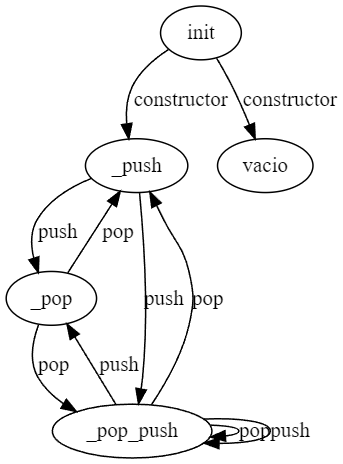
\includegraphics[width=\textwidth]{figs/bounded-stack-good-epa.png}}
        \caption{Enabledness Preserving Abstraction del contrato \texttt{BoundedStack}}
        \label{fig:bounded-stack-epa}
    \end{subfigure}
    \hfill
    \begin{subfigure}{0.45\textwidth}
        {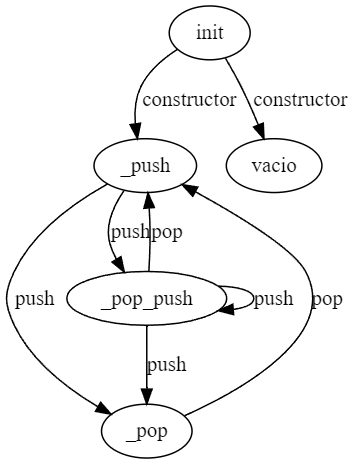
\includegraphics[width=\textwidth]{figs/bonded-stack-bad-epa.png}}
        \caption{EPA errónea del contrato \texttt{BoundedStack} generada por el algoritmo alternativo.
            No se encuentran presentes las transiciones \textbf{\_pop} a \textbf{\_push\_pop} mediante \textcolor{orange}{\texttt{pop}} ni \textbf{\_push\_pop} a \textbf{\_push\_pop} mediante \textcolor{orange}{\texttt{pop}}.}
        \label{fig:bounded-stack-bad-epa}
    \end{subfigure}
\end{figure}


\chapter{Implementación}
Toda esta sección queda anémica y siento que dice cosas o no muy interesantes o de las que no tenemos tanto que decir.
Me parece más bien un punteo de temas que se podrían mencionar que un draft de una versión a incluir verdaderamente.

\section{Algoritmo clásico}
Para implementar el algoritmo clásico de construcción de EPAs necesitamos lo siguiente:
\begin{itemize}
    \item Obtener la lista de métodos y de precondiciones de un contrato
    \item Poder definir estados de un contrato que sean totalmente genéricos y garantizen el invariante \footnote{que no se entiende ``genérico'', pero como lo digo?}
    \item Poder ejecutar los métodos y precondiciones del contrato de manera aislada
    \item Poder ejecutar el invariante del contrato de manera aislada
    \item Realizar consultas sobre el resultado de la ejecución de estos
\end{itemize}
Afortunadamente, la API de Manticore de los contratos inteligentes deployeados ofrece acceso a la lista de sus métodos de manera nativa.
Sin embargo, dado que la abstracción de estos es a nivel bytecode, no resultaba posible extraer de manera automática las precondiciones.
Por otro lado, como mencionamos en la sección \ref{sec:api-manticore} la API programable sólo nos permite generar estados a partir de la ejecución directa de métodos a instancias desde el constructor inicial.
Estas dos limitaciones significaron que tuvimos que introducir las precondiciones como métodos explícitos a los contratos de manera manual, y que necesitamos introducir alguna forma de simular la ejecución de los métodos en el vacío.

Debido al alcance previsto para la experimentación con la herramienta, y para mantener el tiempo de desarrollo al mínimo, optamos por no automatizar la extracción de precondiciones de los métodos en métodos independientes, sino que se realizó de manera totalmente manual en los contratos con los que experimentamos.
De todas formas, debido a que los contratos inteligentes incluyen sus precondiciones de manera explícita al comienzo de los métodos, esta traducción manual consistió en copiar las secciones relevantes y reemplazar las apariciones de \textcolor{magenta}{\texttt{require}} por \textcolor{magenta}{\texttt{return}}.
Luego, para identificar estos métodos automáticamente desde Manticore, establecimos la convención de nomenclatura de introducirles el sufijo \textcolor{orange}{\texttt{\_precondition}}.
Por ejemplo, el método que implementa la preconidición explícita del método \textcolor{orange}{\texttt{MakeOffer}} se llamaría \textcolor{orange}{\texttt{MakeOffer\_precondition}}.

Para poder emular la ejecución de los métodos de manera aislada, era necesario poder construir dentro de Manticore estados (es decir, valores para las variables de la blockchain y las variables de estado) completamente genéricos.
Dado que la API de Manticore sobre los contratos no provee acceso directo a las variables o el storage de los contratos (sólo permite interacturar con los métodos y el estado de la blockchain), decidimos solucionarlo modificando los valores de las variables externamente mediante métodos.
Para esto, también consideramos que lo más veloz en tiempo de desarrollo \footnote{acá la sugerencia es que esto no va, pero uno o dos parráfos más arriba dijimos lo mismo y estaba bien ¿?} sería introducir manualmente un método externo, ``\textcolor{orange}{\texttt{setter}}'', al contrato que recibe un parámetro por cada variable de estado en el contrato, y que asigna el valor recibido a esta.
De esta manera, ejecutar \textcolor{orange}{\texttt{setter}} con parámetros simbólicos genera un estado genérico del contrato.

Los estados resultantes de este proceso, al ser totalmente genéricos, no garantizaban el invariante.
Para reintroducir esta propiedad luego de llamar al \textcolor{orange}{\texttt{setter}} del contrato, aprovechamos la interfaz del módulo \texttt{\textbf{smtlib}} de Manticore.
Lo más sencillo fue introducir el invariante como método explícito de manera manual sólo en el código fuente de los contratos.
Luego usamos este método para restringir los estados genéricos sobre su resultado, de manera análoga a como usamos las implementaciones de las precondiciones.
Los invariantes a lo largo del desarrollo fueron producidos de manera manual para cada contrato, razonando artesanalmente sobre las variables de estado del contrato y como sus métodos las modificaban.

\section{Algoritmo alternativo}
No tengo mucho para decir más allá de lo que ya dijimos hasta ahora.
Cómo pudimos hacer snapshots del estado de un programa en Manticore para poder rollbackear sin tener que generar todo el estado de vuelta no lo mencioné en ningún lado.
La funcionalidad de agregar predicados custom también siento que va acá.

\section{Otros acercamientos}
\subsection{Manticore como caja negra}
En 2023 torres et al. utilizó verisol, una herramienta de bounded model checking sobre contratos Solidity, como caja negra para la construcción de EPAs de smart contracts \cite{torres} \cite{verisol}.
Este approach consiste en codificar las queries de cada transición de la EPA en métodos de un smart contract.
Como mencionamos en la seccion \ref{sec:algoritmo-clasico}, esta query puede traducirse a una consulta de alcanzabilidad de código.
Por ejemplo, en un contrato con tres métodos: \textcolor{magenta}{\texttt{A}}, \textcolor{magenta}{\texttt{B}} y \textcolor{magenta}{\texttt{C}} sin parámetros, para consultar si se puede transicionar desde $\mathcal{M}=\{\textcolor{magenta}{\texttt{A}}, \textcolor{magenta}{\texttt{B}}\}$ a $\mathcal{N} = \{\textcolor{magenta}{\texttt{A}}, \textcolor{magenta}{\texttt{C}}\}$ mediante un llamado a \textcolor{magenta}{\texttt{A}}, el método construido era el siguiente:
\begin{lstlisting}[language=Solidity]
function ABnotC_AnotBC_viaA() public returns (bool) {
    if(A_precondition() && B_precondition() && !C_precondition()){
        A();
        if(A_precondition() && !B_precondition() && C_precondition()){
            assert(false);
        }
    }
}
\end{lstlisting}

Aquí, la alcanzabilidad del \texttt{\textcolor{blue}{\textbf{assert}}(\textcolor{blue}{\textbf{false}})} significaba la existencia de esta transición.
Intentamos utilizar el mismo procedimiento para encontrar las transiciones en la EPA con Manticore, utilizando la herramienta por línea de comandos y la herramienta \texttt{manticore-verifier}.
Sin embargo, la estrategia de exploración de estas dos herramientas era muy poco sofisticada, y no resultaba capaz de encontrar transiciones incluso para contratos muy simples.
Además, la herramienta \texttt{manticore-verifier} tenía comportamiento \textit{buggy} para contratos simples \footnote{``poner un ejemplo''. ¿Pero esto es interesante?}.

\subsection{Abstracción de los contratos por combinación de enums}
Otro método que intentamos para construir las abstracciones de los contratos inteligentes fue no construir las abstracciones en base a predicados sobre las precondiciones, como las EPAs, sino en particionar los estados del contrato en base a los valores que tomaran sus variables de instancia de tipo \textcolor{cyan}{\texttt{enum}}.
A menudo los contratos inteligentes están diseñados considerando una cantidad finita de configuraciones posibles, como si se abstrayeran a una máquina de estados finita particular.
Estos contratos están programados haciendo uso de variables de estado de tipo \textcolor{cyan}{\texttt{enum}} que indican el estado en el que se encuentra el contrato con respecto a diversas propiedades, a menudo indicando propiedades independientes con distintas variables.

Consideremos el siguiente ejemplo, el contrato \texttt{RoomThermostat} del benchmark ``Microsoft Azure Blockchain Workbench'' \cite{azure-benchmark} que podemos ver en la figura \ref{fig:rooomthermostat-solidity}.
Como mencionamos, hace uso de las variables de tipo \textcolor{cyan}{\texttt{enum}} para indicar los estados de ejecución en los que se encuentra el contrato.
En particular, la variable \texttt{State} controla el acceso a cada uno de los métodos del contrato, mientras que la variable \texttt{Mode} indica otras propiedades relevantes del estado contrato.
De los métodos disponibles, podemos ver que los métodos \textcolor{orange}{\texttt{SetMode}} y \textcolor{orange}{\texttt{SetTargetTemperature}} se encuentran habilitados cuando el valor de \texttt{State} es \texttt{InUse}, mientras que el método \textcolor{orange}{\texttt{StartThermostat}} requiere que el valor de \texttt{State} sea \texttt{Created}.

\begin{lstlisting}[language=Solidity, label={fig:rooomthermostat-solidity}, caption={Contrato Inteligente \texttt{RoomThermostat} en Solidity},captionpos=b]
pragma solidity >=0.4.25 <0.6.0;
contract RoomThermostat
{
    //Set of States
    enum StateType { Created, InUse}
    
    //List of properties
    StateType public State;
    address public Installer;
    address public User;
    int public TargetTemperature;
    enum ModeEnum {Off, Cool, Heat, Auto}
    ModeEnum public  Mode;
    
    constructor(address thermostatInstaller, address thermostatUser) public
    {
        Installer = thermostatInstaller;
        User = thermostatUser;
        TargetTemperature = 70;
    }

    function StartThermostat() public
    {
        if (Installer != msg.sender || State != StateType.Created)
        {
            revert();
        }

        State = StateType.InUse;
    }

    function SetTargetTemperature(int targetTemperature) public
    {
        if (User != msg.sender || State != StateType.InUse)
        {
            revert();
        }
        TargetTemperature = targetTemperature;
    }

    function SetMode(ModeEnum mode) public
    {
        if (User != msg.sender || State != StateType.InUse)
        {
            revert();
        }
        Mode = mode;
    }
}
\end{lstlisting}

Siguiendo esta idea, consideramos generar abstracciones donde los estados están definidos por las posibles combinaciones de las variables de estado de tipo \textcolor{cyan}{\texttt{enum}}, confiando en cada distinta combinación	de estas variables se corresponde con un estado de ejecución único del contrato interesante.
En estas abstracciones consideramos que las transiciones sean por los métodos externos del contrato, al igual que en las EPAs.

Continuando el ejemplo del contrato \texttt{RoomThermostat}, en la figura \ref{fig:room-thermostat-states} podemos ver la abstracción resultante.
Si prestamos atención a la variable \texttt{State}, vemos que la máquina de estados se divide en dos secciones:
Por un lado los estados etiquetados como \texttt{InUse} presentan transiciones por los métodos \textcolor{orange}{\texttt{SetMode}} y \textcolor{orange}{\texttt{SetTargetTemperature}}.
Por otro lado el único estado etiquetado como \texttt{Created} tiene una única transición, que ocurre por el método \textcolor{orange}{\texttt{SetMode}}.
Además, el conjunto de estados etiquetados con \texttt{InUse} están particionados por la variable \texttt{Mode}, pudiendo transicionar entre cualquiera de los estados al ejecutar el método \textcolor{orange}{\texttt{SetMode}}.
En cambio ejecutar el método \textcolor{orange}{\texttt{SetTargetTemperature}}, que solo afecta variables internas que no son de tipo \textcolor{cyan}{\texttt{enum}}, siempre resulta en una transición al mismo estado desde el que se lo ejecutó.

\begin{figure}[H]
    \centering
    {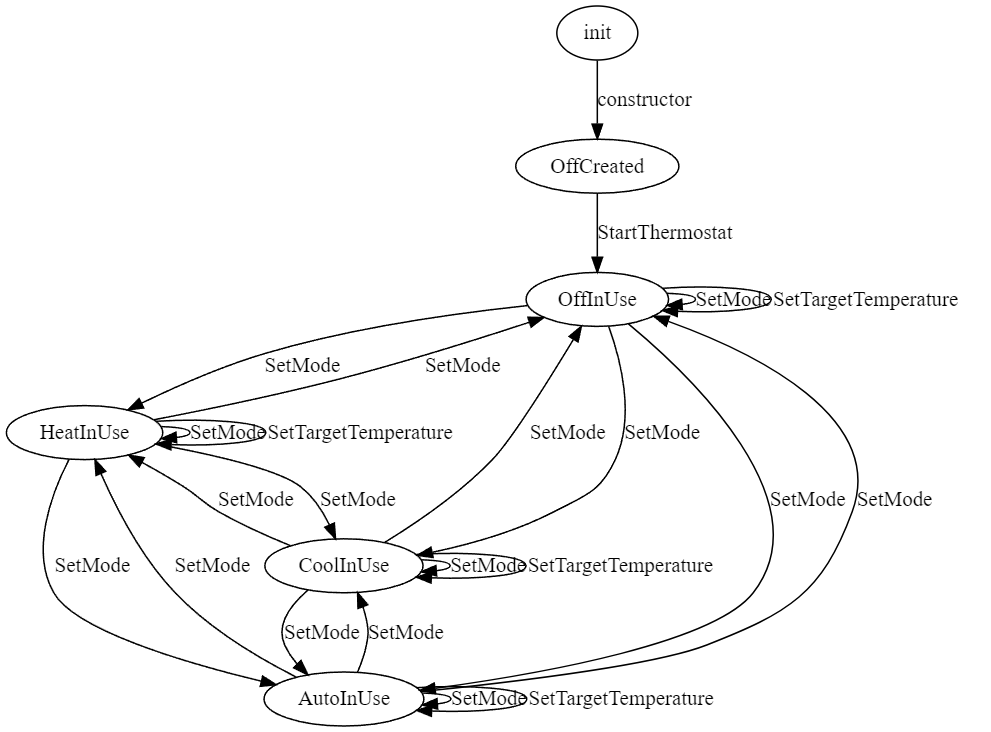
\includegraphics {figs/room-thermostate-abstraction.png}}
    \caption{Abstracción por estado de las variables \textcolor{cyan}{\texttt{enum} del contrato \texttt{RoomThermostat}}}
    \label{fig:room-thermostat-states}
\end{figure}

A la hora de implementar la generación de estas abstracciones, para poder utilizar el mismo mecanismo de generación de abstracciones que el utilizado para las EPAs era necesario conocer el valor de las variables de instancia de tipo \textcolor{cyan}{\texttt{enum}}.
Aquí, nuevamente por consideraciones en el tiempo de desarrollo \footnote{¿Acá también está mal hablar de eso?}, lo mas sencillo fue tratar la introspección de estas variables de manera similar a los valores de las precondiciones de los métodos.
Lo que hicimos fue definir métodos externos para cada una de las variables de instancia de tipo \textcolor{cyan}{\texttt{enum}} que permitieran observar el valor de esta variable.
Luego, podíamos detectar estos métodos introduciendo un nuevo tipo sufijo ``\textcolor{orange}{\texttt{\_enum}}''.
Por ejemplo, para la variable \texttt{Mode} en el contrato \texttt{RoomThermostat}, el método generado era el siguiente:

\begin{lstlisting}[language=Solidity]
    function Mode_enum() public returns (ModeEnum) {
        return Mode;
    }
\end{lstlisting}

Utilizando estos nuevos métodos externos el mecanismo era el mismo, con la diferencia de que los estados se construían tomando combinaciones de los \textcolor{cyan}{\texttt{enum}} en lugar de de las precondiciones


\chapter{Análisis}
En esta sección realizamos algunos análisis sobre el comportamiento y performance de los prototipos implementados.
Primero realizamos una evaluación manual de la calidad de las abstracciones generadas por el algoritmo clásico y el alternativo.
Luego, evaluamos el tiempo empleado en promedio de cada algoritmo sobre un benchmark conocido y por último realizamos un análisis sobre cuáles son las partes más costosas en tiempo del prototipo implementado.

Los análisis fueron realizados sobre el benchmark \textit{Microsoft Azure Blockchain Workbench} \cite{azure-benchmark}, un benchmark conocido para el cual ya contabamos con las EPAs correctas debido a que fue utilizado en \cite{predicate-abstraction-for-smart-contract-validation} \cite{torres}.
Además, realizamos algunos estudios sobre el contrato \texttt{BoundedStack} presentado en la sección \ref{code:solidity-bounded-stack}.
Los contratos analizados fueron los siguientes:

\begin{center}
    \begin{tabular}{|l|c|c|}
        \hline
        \textbf{Contrato}         & \textbf{Lineas de codigo} & \textbf{Cantidad de estados de la EPA} \\
        \hline
        DefectiveComponentCounter & 33                        & 2                                      \\
        \hline
        SimpleMarketplace         & 66                        & 4                                      \\
        \hline
        BasicProvenance           & 48                        & 3                                      \\
        \hline
        RoomThermostat            & 48                        & 3                                      \\
        \hline
        BoundedStack              & 28                        & 5                                      \\
        \hline
    \end{tabular}
\end{center}

Los experimentos se efectuaron en una máquina con un procesador Intel Core i7-4770 \@ 3,40GHz x 8, 16 GB RAM, Mesa Intel HD Graphics4600 (HSW GT2) y almacenamiento SSD 256 GB, ejecutando Ubuntu 22.04.3 LTS.

\section{Comparación de las abstracciones generadas entre el algoritmo clásico y el alternativo}
Como mencionamos en la sección \ref{sec:subaproximacion}, las abstracciones generadas por el algoritmo alternativo no siempre son Enabledness Preserving Abstractions\footnote{Es decir, en algunos casos no cumplen la definición presentada en la sección \ref{definicion-epa}.} de los contratos analizados, sino que son unas subaproximaciones de estas.
Al mismo tiempo, las EPAs son sobreaproximaciones del comportamiento de los contratos, por lo que el mecanismo resultante del algoritmo alternativo yace en algún lugar intermedio: no es ni sound ni complete.
Por esto, nos interesa explorar en particular cuáles son las diferencias producidas entre el algoritmo alternativo y las generadas por el algoritmo clásico (las EPAs) para evaluar su utilidad.
Para responder estas preguntas analizamos el desempeño de los prototipos implementados usando ambos algoritmos sobre algunos casos de prueba.

\subsection{Caso \texttt{RoomThermostat}}
El primer caso que evaluamos fue el contrato \texttt{RoomThermostat}, cuyo código fuente podemos ver en el fragmento de código \ref{fig:rooomthermostat-solidity}.
Es un contrato pequeño, con pocos métodos y un invariante sencillo.
Para poder emplear el algoritmo clásico sobre este contrato, el invariante propuesto fue el siguiente:
\begin{lstlisting}[language=Solidity]
    function invariant(StateType stateNew, address installerNew, address userNew, int targetTemperatureNew, ModeEnum modeNew) public returns(bool){
        bool result = (stateNew == StateType.Created || stateNew == StateType.InUse);
        result = result && (modeNew == ModeEnum.Auto || modeNew == ModeEnum.Cool || modeNew == ModeEnum.Heat || modeNew == ModeEnum.Off);
        if(stateNew == StateType.Created){
            result = (targetTemperatureNew == 70) && (modeNew == ModeEnum.Off);
        }
        return result;
    }
\end{lstlisting}

Luego, evaluamos tanto el algoritmo clásico como el alternativo sobre el contrato.
En ambos casos la EPA generada fue la misma, una máquina de estados sencilla de tan sólo tres estados que podemos ver en la figura \ref{fig:room-thermostat-epa}.

\begin{figure}
    \centering
    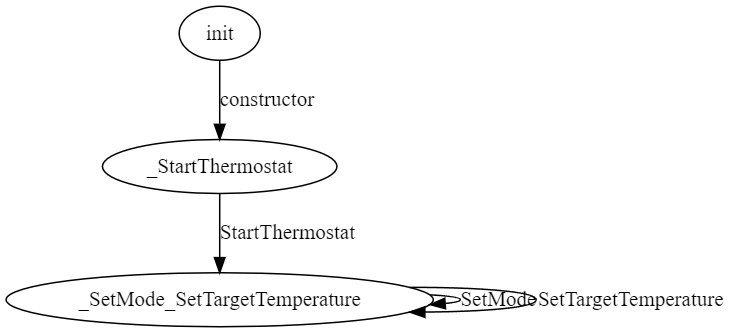
\includegraphics[width=0.75\textwidth]{figs/room-thermostate-epa.png}
    \caption{Enabledness Preserving Abstraction del contrato \texttt{RoomThermostat} }
    \label{fig:room-thermostat-epa}
\end{figure}

\subsection{Caso \texttt{BoundedStack}}
El siguiente caso que evaluamos fue el ejemplo teórico que expusimos en la sección \ref{sec:subaproximacion}, el contrato \texttt{BoundedStack}, con intención de evidenciar las subaproximaciones realizadas por el algoritmo nuevo.
El código del contrato se encuentra en el fragmento de código \ref{code:solidity-bounded-stack}.
Nos interesa corroborar el comportamiento de ambos algoritmos, si se produce alguna subaproximación, y cuáles.

Lo primero que vimos al evaluar la abstracción generada por el algoritmo alternativo sobre el contrato \texttt{BoundedStack} lo podemos ver en la imagen \ref{fig:buggy-bounded-stack-epa}.
En esa abstracción  podemos ver que faltan algunas de las transiciones presentes en la EPA del contrato, pero además podemos observar que las transiciones por \textcolor{orange}{\texttt{pop}} siempre llevan al estado desde el que se ejecutó el método.
Cuando realizamos esta comparación, esta observación generó bastante confusión, hasta que comprendimos que se debía a un defecto en el código fuente de \texttt{BoundedStack} que no decrementaba la variable \texttt{size} al ejecutar \textcolor{orange}{\texttt{pop}}.
Luego de corregir el defecto, la abstracción generada por el prototipo fue la referenciada en la imagen \ref{fig:bounded-stack-bad-epa}.
Es decir, la misma que elaboramos durante el ejemplo teórico del comportamiento del algoritmo alternativo, y la que evidenciaba la falencia del algoritmo alternativo para este ejemplo.
Decidimos incluir este pequeña caso de un error en el código fuente en lugar de omitirlo para ejemplificar que, a pesar de que quede evidenciado que el algoritmo nuevo genere subaproximaciones de las EPAs en la práctica, las abstracciones generadas pueden seguir resultando útiles a la hora de atrapar errores.

\begin{figure}[H]
    \centering
    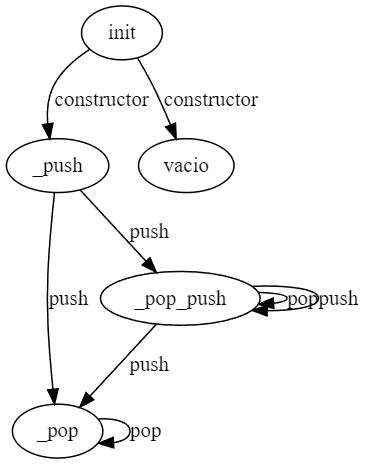
\includegraphics[width=0.45\textwidth]{figs/buggy-bounded-stack-epa.png}
    \caption{Enabledness Preserving Abstraction del contrato \texttt{BoundedStack} con un error que no decrementa el tamaño luego de ejecutar \textcolor{orange}{\texttt{pop}} }
    \label{fig:buggy-bounded-stack-epa}
\end{figure}

A la hora de emplear el algoritmo clásico sobre el contrato, el invariante propuesto fue el siguiente:
\begin{lstlisting}[language=Solidity]
    function invariant() public returns(bool){
        bool result = (size >= 0) && (size <= maxSize);
        result = result && (internal_arr.length == size);
        return result;
    }
\end{lstlisting}

Sin embargo, el prototipo desarrollado con el algoritmo clásico no pudo analizar este contrato satisfactoriamente, sino que terminó el analisis por time out luego de 24 horas.
Esto se debe a que el paso de restringir las instancias del contrato a aquellas que satisfagan el invariante resultó demasiado difícil para el motor de ejecucion simbólica de Manticore.
Algunos experimentos y análisis intermedios nos hacen creer que se debe a la pobre representación de las variables de tipo \textcolor{cyan}{\texttt{uint256[]}} del mismo.
Esto significó que terminamos el análisis comparando la abstracción generada por el algoritmo alternativo no con la generada por el algoritmo clásico, sino con una EPA producida manualmente.

\section{Comparación en tiempo de ejecución entre el algoritmo clásico y el alternativo}
Otra hipótesis generada durante el desarrollo del algoritmo alternativo fue que el evitar la ejecución de los invariantes mejoraría el tiempo de ejecución.
Esto se debe a que los invariantes, comparados con las precondiciones de los métodos externos, son propiedades relativamente complejas que además pueden hablar sobre el estado de variables internas de tipos complejos como arrays, mappings, etc.
Para evaluar esta hipótesis estudiamos el tiempo de ejecución empleado por los prototipos que implementan el algoritmo alternativo y el clásico en Manticore.

Ya que el benchmark que utilizamos había sido utilizado por Godoy et al. en 2022 \cite{predicate-abstraction-for-smart-contract-validation}, a la hora de experimentar contamos con EPAs de todos los contratos involucrados, por lo que además pudimos usarlas para corroborar la correctitud de las abstracciones generadas.
Los experimentos fueron realizados ejecutando ambos prototipos sobre cada contrato cinco veces y luego tomando el promedio del tiempo total de ejecución.

En la figura \ref{fig:classic-vs-alternativo} podemos ver los resultados del experimento realizado.
Las mediciones fueron solo realizadas para los contratos \texttt{DefectiveComponentCounter}, \texttt{RoomThermostat}, \texttt{BasicProvenance} y \texttt{SimpleMarketplace} porque como podemos ver el tiempo de ejecución de la implementación del algoritmo clásico nunca fue menor a diez horas.
A pesar de que en todos los contratos analizados podamos ver una diferencia significativa al emplear el algoritmo alternativo, es importante destacar que los tiempos de ejecución de esta técnica aún se mantuvieron muy altos.
La mejora en tiempo parecería ser relativamente constante a lo largo de los cuatro contratos analizados, habiendo tardado el algoritmo alternativo alrededor de diez horas menos que el clásico.
Esta diferencia cercana a constante posiblemente se deba a que todos los contratos eran muy simples, por lo que no se pudo observar la diferencia en comportamiento que habría en contratos más complejos.

\begin{figure}[h]
    \centering
    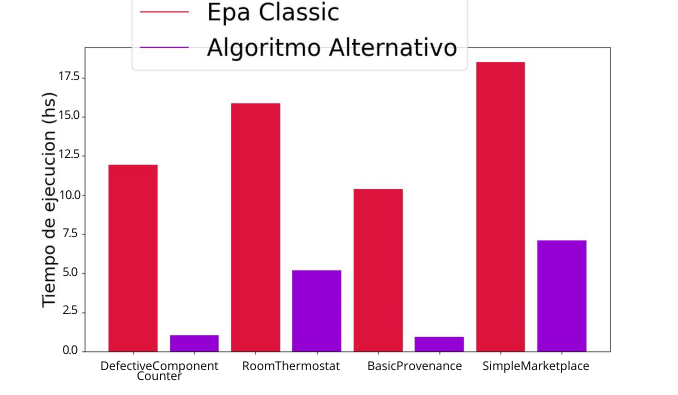
\includegraphics[width=0.65\textwidth]{figs/classic_vs_alternativo.png}
    \caption{Tiempo promediado para 5 ejecuciones (en horas) de la generación de abstracciones del prototipo que implementa el algoritmo alternativo y el algoritmo clásico}
    \label{fig:classic-vs-alternativo}
\end{figure}

A pesar de que la mejora del algoritmo alternativo frente al clásico fuese tan grande, los valores obtenidos con el algoritmo alternativo siguieron sin resultar razonables.
Si observamos los valores obtenidos, el tiempo de cómputo en promedio fue de entre media hasta casi ocho horas, lo que no resulta aplicable para un usuario de la herramienta que pretende generar las abstracciones en tiempo real.
Por este motivo decidimos realizar los experimentos que mostraremos a continuación, en los que buscamos conseguir mejoras en el tiempo de ejecución o claridad en la razón de que tarde tanto.


\section{Evaluación más detallada del tiempo de ejecución del algoritmo alternativo}
Para mejorar el tiempo de ejecución del prototipo buscamos identificar en qué partes del análisis era que se consumía la mayor parte del tiempo empleado.
Lo primero que hicimos fue identificar ``etapas'' en el algoritmo alternativo que pudimos diferenciar para medir el tiempo empleado en cada una de ellas.
Por otro lado analizamos el código fuente de Manticore y diferenciamos en distintos niveles de abstracción las funcionalidades que estábamos usando.

La separación de la ejecución del algoritmo en etapas la hicimos en estas dos:
\begin{enumerate}
    \item La ejecución simbólica de los métodos \footnote{Al desplegado simbólico del contrato lo consideramos parte de la ejecución simbólica de los métodos.}
    \item La solución de queries de satisfacibilidad sobre las transiciones en la EPA
\end{enumerate}
Refiriéndonos al algoritmo alternativo, podemos ver que este alterna entre estas dos etapas.
Nos resulta de interés ver cuál, si alguna, consume la mayor parte del tiempo de ejecución.

A continuación indicamos cuál fue la división en niveles de abstracción que hicimos de las funcionalidades de Manticore.
En particular, por como es la arquitectura de multithreading y \textbf{\texttt{workers}} de Manticore, solo pudimos hacer esta distinción en los métodos relacionados a la resolución de valores simbólicos.
La manera en la que se realizaba la ejecución simbólica y la generación de las condiciones de camino era demasiado dependiente de objetos creados dinámicamente como para poder ser analizada de la misma manera.
\begin{enumerate}
    \item \textbf{Nivel Externo}\footnote{En el momento de realizar las mediciones, los valores para este nivel se registraron bajo el nombre de  ``Nivel 3''} : utilizado para medir el tiempo que consumían las funciones de la API de manticore que nuestro prototipo llamaba directamente.
          La única función cuyo tiempo medimos en este nivel fue \texttt{generateTestCases}.
    \item \textbf{Nivel \texttt{state}} : Utilizado en las funciones del módulo \textbf{\texttt{state}} que identificamos que eran llamadas.
          Los métodos registrados bajo este nivel fueron \texttt{can\_be\_true} y \texttt{solve\_\allowbreak one\_\allowbreak n\_\allowbreak batched}.
    \item \textbf{Nivel SMT solver} : Utilizado alrededor de cada llamado directo al SMT solver en los métodos del módulo \textbf{\texttt{smtlib}}.
          Los métodos registrados bajo este nivel fueron \texttt{\_is\_sat}, \texttt{\_get\_value} y \texttt{\_\_get\_value\_all}.
\end{enumerate}
Cada uno de los métodos fue modificado para medir el tiempo empleado entre el principio y el fin de la zona delimitada de interés.
Por ejemplo, en el fragmento de códgio \ref{code:getvalueall-modification} podemos ver los cambios introducidos en el método \texttt{\_\_get\_value\_all} del \textbf{Nivel SMT solver} para registrar el tiempo.

\begin{lstlisting}[language=Python,
    label={code:getvalueall-modification},
    caption={Método \texttt{\_\_get\_value\_all} del modulo \textbf{\texttt{smtlib}} modificado para registrar el tiempo empleado por la llamada al SMT solver.
    El código resaltado indica las líneas agregadas para registrar el tiempo.},
    captionpos=b]
def __getvalue_all(self, expressions_str: List[str], is_bv: List[bool]) -> Dict[str, int]:
    (*@| \hl{start = time.time()} |@*)
    all_expressions_str = " ".join(expressions_str)
    self._smtlib.send(f"(get-value ({all_expressions_str}))")
    ret_solver: Optional[str] = self._smtlib.recv()
    (*@| \hl{print}|@*)(f"(level _getvalue_all_z3_call) took {time.time()- start} seconds")
    assert ret_solver is not None
    return_values = re.findall(RE_GET_EXPR_VALUE_ALL, ret_solver)
    
    return {value[0]: _convert(value[1]) for value in return_values}
\end{lstlisting}

De  entre los métodos a los que les registramos el tiempo de ejecución, sabíamos que los métodos en \textbf{Nivel Externo} solo eran ejecutados cuando el prototipo implementado los llamaba explícitamente.
Por otro lado, los métodos en \textbf{Nivel \texttt{state}} eran métodos que a veces eran llamados desde la implementación directamente, pero además eran ejecutados como métodos internos de otros procesos durante el análisis.
Por último, los métodos del \textbf{Nivel SMT solver} eran ejecutados en diversos momentos del análisis.

Una vez hecha esta separación en etapas del algoritmo y niveles de abstracción, medimos el tiempo total en promedio empleado por cada etapa y cada nivel de abstracción.
Por otro lado, además, calculamos para cada uno de los niveles de abstracción la cantidad de veces que este mismo fue registrado y el tiempo total empleado.
Esto fue para intentar percibir discrepancias entre los niveles que esperábamos que consumieran la mayoría del tiempo y lo que pudiéramos medir.

\begin{figure}
    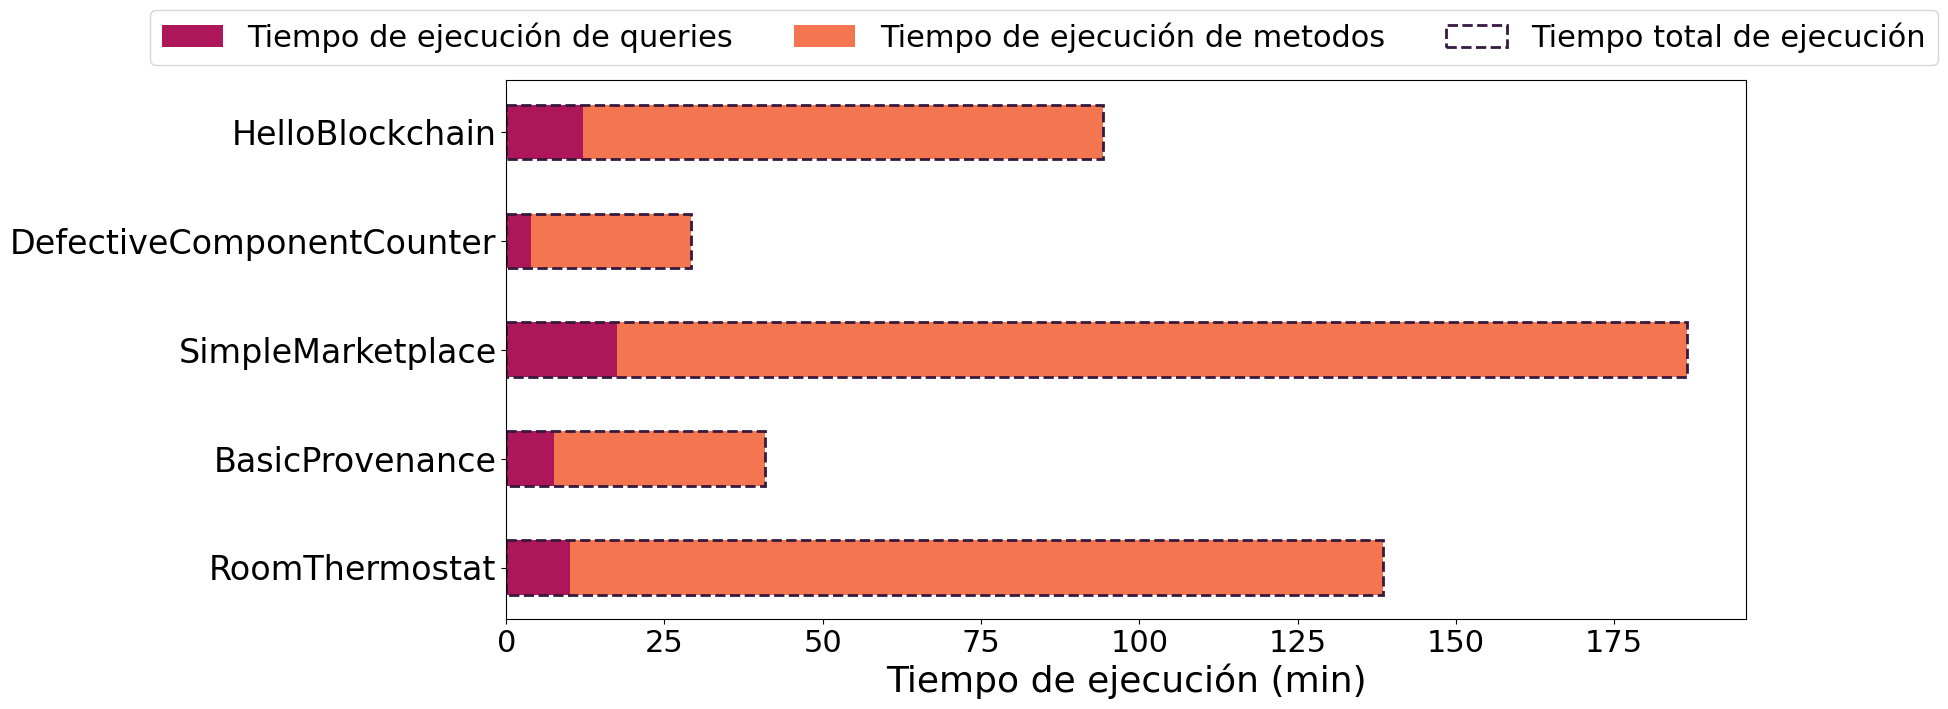
\includegraphics[width=\textwidth]{figs/categories-bar-graph.png}
    \caption{Proporción del tiempo de ejecución promediado entre 5 (en horas) del algoritmo alternativo.
        En naranja el tiempo empleado por la ejecución simbólica de los métodos, en violeta por la resolución de queries de predicados y en líneas punteadas el tiempo total (medido) empleado por el algoritmo.}
    \label{fig:tiempo-categorias}
\end{figure}

En la figura \ref{fig:tiempo-categorias} podemos ver las mediciones obtenidas sobre el tiempo empleado por las dos etapas del algoritmo.
Se ve que la gran mayoría del tiempo empleado durante la generación de EPAs con el algoritmo involucrado fue consumido por la ejecución simbólica de los métodos.
La resolución de predicados para consultar por la presencia de transiciones en la EPA, en cambio, fue comparativamente pequeña.
Por ejemplo, para el contrato \texttt{BasicProvenance}, podemos ver que a pesar que el promedio del tiempo total fue cercano a los 40 minutos, la etapa de resolución de queries demoró tan sólo valores cercanos a los 7 minutos.
Por otro lado, la suma del tiempo empleado en promedio por ambas etapas resulta a simple vista idéntico al tiempo total promedio que se pudo medir, por lo que tampoco observamos un consumo inusualmente alto de tiempo por algún otro aspecto del análisis que no hayamos considerado.

En las tablas \ref{tab:performance-DefectiveComponentCounter} a \ref{tab:performance-BasicProvenance} podemos ver los resultados obtenidos en las mediciones del tiempo empleado en cada nivel de abstracción de los métodos de Manticore para los contratos.
Podemos ver en la tabla \ref{tab:performance-BasicProvenance} los valores obtenidos para el contrato \texttt{BasicProvenance},
en el que nos queremos enfocar primero, para señalar las relaciones entre los valores para algunos de los métodos.
Haciendo memoria sobre el análisis de la figura \ref{fig:tiempo-categorias}, podemos ver que los aproximadamente 450 segundos empleados por el método \texttt{generateTestCases}, que es el más externo de todos, representan casi la totalidad (7.5 minutos) del tiempo empleado por la etapa de solución de queries del programa.
De hecho, los métodos \texttt{solve\_one\_n\_batched} y \texttt{get\_value\_in\_batch}, que pertenecen a un nivel de abstracción menor, siguen siendo responsables por la mayoría del tiempo empleado (y si observamos el número de veces que cada uno fue llamado, a fines del análisis que estamos haciendo ambos métodos resultan prácticamente iguales).
Sin embargo, al realizar el salto a los métodos de \textbf{Nivel SMT solver}, vemos que comparativamente estos casi ni aportaron al tiempo empleado.
Los tres métodos \texttt{\_getvalue\_all}, \texttt{\_is\_sat} y \texttt{\_getvalue}, todos llamados de manera directa por los métodos del nivel superior, apenas aportan 5 segundos de los 7.5 minutos involucrados.

Por otro lado, notamos que esta relación entre los métodos de los tres niveles de abstracción se preserva para los otros contratos (tablas \ref{tab:performance-DefectiveComponentCounter}, \ref{tab:performance-SimpleMarketplace} y \ref{tab:performance-RoomThermostat}) también: los métodos \texttt{generateTestCases}, \texttt{solve\_one\_n\_batched} y \texttt{get\_value\_in\_batch} consumen casi la totalidad del tiempo empleado mientras que los metodos del \textbf{Nivel SMT Solver} no consumen casi nada.
De aquí podemos intentar obtener dos conclusiones.
O bien las llamadas al SMT solver funcionan de una manera asincrónica, que no pudimos capturar en nuestras mediciones, o bien en efecto la mayoría del tiempo consumido por consultas a Manticore es empleado no en tiempo de procesamiento del SMT solver, sino en alguna etapa de la aplicación misma (que no fuimos capaces de medir).
Considerando que la mayor parte del tiempo de ejecución de la aplicación fue consumido por la etapa de ejecución simbólica, y no por la de resolución de queries, es posible que el preprocesamiento de las condiciones simbólicas de Manticore, construido durante la etapa de ejecución simbólica, sea extraordinariamente complejo y por ende caro en tiempo de ejecución.
Además, un rudimentario y primer análisis del código involucrado sugiere que los llamados realizados al SMT solver son completamente sincrónicos, aunque no se pudo realizar un experimento para corroborar ninguna de estas dos hipótesis.


% Define custom colors
\definecolor{color1}{rgb}{0.9, 0.9, 0.9} % Light gray
\definecolor{color2}{rgb}{0.8, 0.8, 0.8} % Medium gray
\definecolor{color3}{rgb}{0.7, 0.7, 0.7} % Dark gray

\begin{table}[ht]
    \begin{minipage}{0.95\textwidth}
        \centering
        \begin{tabular}[t]{l @{\hskip 30pt} r @{\hskip 30pt} r}
            \toprule
            \textbf{Método de Manticore}                      & \textbf{Número de llamados} & \textbf{Tiempo empleado (s)} \\
            \midrule
            \rowcolor{color1} \texttt{\_getvalue}             & 4                           & 0.00188                      \\
            \rowcolor{color1} \texttt{\_is\_sat}              & 80                          & 0.48341                      \\
            \rowcolor{color2} \texttt{state.can\_be\_true}    & 21                          & 0.21036                      \\
            \rowcolor{color1} \texttt{\_getvalue\_all}        & 30                          & 1.62389                      \\
            \rowcolor{color2} \texttt{get\_value\_in\_batch}  & 54                          & 230.79537                    \\
            \rowcolor{color2} \texttt{solve\_one\_n\_batched} & 54                          & 231.65494                    \\
            \rowcolor{color3} \texttt{generateTestCases}      & 3                           & 231.87251                    \\
            \bottomrule
        \end{tabular}
        \caption{Tiempo empleado por los métodos de Manticore para el contrato \texttt{DefectiveComponentCounter}.}
        \label{tab:performance-DefectiveComponentCounter}
    \end{minipage}
    \begin{minipage}{0.95\textwidth}
        \centering
        \begin{tabular}[t]{l @{\hskip 30pt} r @{\hskip 30pt} r}
            \toprule
            \textbf{Método de Manticore}                      & \textbf{Número de llamados} & \textbf{Tiempo empleado (s)} \\
            \midrule
            \rowcolor{color1} \texttt{\_getvalue}             & 110                         & 2.16616                      \\
            \rowcolor{color1} \texttt{\_is\_sat}              & 370                         & 9.89551                      \\
            \rowcolor{color2} \texttt{state.can\_be\_true}    & 61                          & 0.63042                      \\
            \rowcolor{color1} \texttt{\_getvalue\_all}        & 55                          & 4.25464                      \\
            \rowcolor{color2} \texttt{get\_value\_in\_batch}  & 84                          & 1028.78724                   \\
            \rowcolor{color2} \texttt{solve\_one\_n\_batched} & 84                          & 1029.55111                   \\
            \rowcolor{color3} \texttt{generateTestCases}      & 4                           & 1030.08048                   \\
            \bottomrule
        \end{tabular}
        \caption{Tiempo empleado por los métodos de Manticore para el contrato \texttt{SimpleMarketplace}.}
        \label{tab:performance-SimpleMarketplace}
    \end{minipage}
    \begin{minipage}{0.95\textwidth}
        \centering
        \begin{tabular}[t]{l @{\hskip 30pt} r @{\hskip 30pt} r}
            \toprule
            \textbf{Método de Manticore}                      & \textbf{Número de llamados} & \textbf{Tiempo empleado (s)} \\
            \midrule
            \rowcolor{color1} \texttt{\_getvalue}             & 249                         & 16.3826                      \\
            \rowcolor{color1} \texttt{\_is\_sat}              & 684                         & 62.46842                     \\
            \rowcolor{color2} \texttt{state.can\_be\_true}    & 89                          & 2.59814                      \\
            \rowcolor{color1} \texttt{\_getvalue\_all}        & 59                          & 3.97965                      \\
            \rowcolor{color2} \texttt{get\_value\_in\_batch}  & 88                          & 583.78606                    \\
            \rowcolor{color2} \texttt{solve\_one\_n\_batched} & 88                          & 584.46269                    \\
            \rowcolor{color3} \texttt{generateTestCases}      & 4                           & 584.95501                    \\
            \bottomrule
        \end{tabular}
        \caption{Tiempo empleado por los métodos de Manticore para el contrato \texttt{RoomThermostat}.}
        \label{tab:performance-RoomThermostat}
    \end{minipage}
    \begin{minipage}{0.95\textwidth}
        \centering
        \begin{tabular}[t]{l @{\hskip 30pt} r @{\hskip 30pt} r}
            \toprule
            \textbf{Método de Manticore}                      & \textbf{Número de llamados} & \textbf{Tiempo empleado (s)} \\
            \midrule
            \rowcolor{color1} \texttt{\_getvalue}             & 62                          & 0.4647                       \\
            \rowcolor{color1} \texttt{\_is\_sat}              & 196                         & 2.24389                      \\
            \rowcolor{color2} \texttt{state.can\_be\_true}    & 21                          & 0.19231                      \\
            \rowcolor{color1} \texttt{\_getvalue\_all}        & 31                          & 2.33352                      \\
            \rowcolor{color2} \texttt{get\_value\_in\_batch}  & 54                          & 449.60244                    \\
            \rowcolor{color2} \texttt{solve\_one\_n\_batched} & 54                          & 450.04921                    \\
            \rowcolor{color3} \texttt{generateTestCases}      & 3                           & 450.27618                    \\
            \bottomrule
        \end{tabular}
        \caption{Tiempo empleado por los métodos de Manticore para el contrato \texttt{BasicProvenance}.}
        \label{tab:performance-BasicProvenance}
    \end{minipage}
    \caption*{Tiempo empleado por los métodos de Manticore involucrados en las queries por transiciones en la EPA para los distintos contratos. En el color más oscuro los métodos del \textbf{Nivel Externo}, en el color intermedio los del \textbf{Nivel \texttt{state}} y en el más claro los del \textbf{Nivel SMT solver}}
\end{table}


\chapter{Conclusiones}

%%%% BIBLIOGRAFIA
\backmatter
\printbibliography


\end{document}
